% ----------------------------------------------------------
\chapter{Introdução}
% ----------------------------------------------------------

A profícua evolução do processamento computacional proporcionou avanços importantes em diversas áreas do conhecimento humano, como o \textit{design} de fármacos, o planejamento sintético e a ciência de materiais, com alto potencial de aplicabilidade. Essa tendência foi observada por Gordon E. Moore \autocite{Mack2011, Shalf2020}, químico estadunidense 
cofundador da \href{https://www.intel.com/content/www/us/en/company-overview/company-overview.html}{\textit{Intel Corporation}}. A partir dele, foi cunhada uma expressão para designar o aumento bianual de 100\% no número de transistores dos chips microprocessadores, pelo mesmo custo. Isso possibilita, de maneira crescente, a implementação de ferramentas capazes de acessar - seja por meio de cálculos de estrutura eletrônica, 
simulações, ou predições - propriedades que não podem ser obtidas experimentalmente de forma direta. Isso faz com que os computadores ocupem um lugar de destaque no estudo fenomenológico dentro da  química \autocite{Allouche2010, Rayan2017}, acessando a escala quântica da matéria através de relações matemáticas.

Nesse sentido, existe uma pungente necessidade de criar novas abordagens de compreensão da química através da visualização molecular tridimensional, que refere-se a um procedimento visual de interação entre a realidade e a teoria a partir de um modelo\footnote{Modelos mentais são dispositivos do pensamento por meio dos quais um ser humano tenta explicar, a si próprio e aos outros, como funciona o mundo real. É um tipo de símbolo interno de representação da realidade externa, hipotética, que tem um papel importante na cognição – ou seja, na forma como apreendemos o mundo.}, seja ele filosófico, mecânico ou computacional \autocite{Snyder2021}, cada qual com sua respectiva aplicação. Por exemplo, os fenômenos físicos envolvendo os núcleos dos átomos e seus elétrons são problemas dinâmicos, de múltiplos corpos, com alta complexidade. Desse modo, nem sempre é possível calcular analiticamente as grandezas de interesse, como a própria energia eletrônica dos sistemas não-hidrogeniônicos.

A interpretação desses fenômenos químicos a partir de informações estruturais auxilia na compreensão, seja ela qualitativa ou quantitativa, dos dados observados no mundo real, como a reatividade, por exemplo. Nesse sentido, a aromaticidade faz-se relevante para realizar análises preditivas, uma vez que a deslocalização eletrônica é um efeito estabilizador que gera consequências na seletividade de reações químicas.

No entanto, encontrar uma definição de aromaticidade que seja curta, formal e inequívoca torna-se um desafio para os químicos, pois esta não é uma grandeza física. Para dirimir tal dificuldade, é possível elencar um conjunto de propriedades observadas em compostos que coincidem ao exibir o mesmo caráter aromático, mas de forma multidimensional, ou seja, que concerne a níveis ou campos variados. Isso nos leva a concluir que a aromaticidade, por não ser uma observável física, pode ser caracterizada através de diferentes critérios (geométricos, energéticos, magnéticos e topológicos) que apresentam certo grau de correlação. Classicamente, a aromaticidade pode ser definida pelo aumento da estabilidade termodinâmica de compostos cíclicos $\pi$-conjugados quando comparados aos seus análogos cujos elétrons são localizados. Essa tendência comprova-se avaliando a entalpia envolvida na hidrogenação ($\Delta H^\circ$) de um alceno catalisada por paládio. Tal processo é sempre exotérmico, isto é, libera uma certa quantidade de calor. Por exemplo, se analisarmos a reação de um cicloexeno (\autoref{fig:1}), o valor numérico do $\Delta H^\circ$ será -28,6 kcal/mol (\autoref{fig:2}). 

%% TODO: adicionar imagem sobre estabilização termodinâmica de compostos aromáticos

\begin{figure}[htb]
	\caption{\label{fig:1} Reação de hidrogenação de um alceno cíclico catalisada por paládio.}
	\begin{center}
		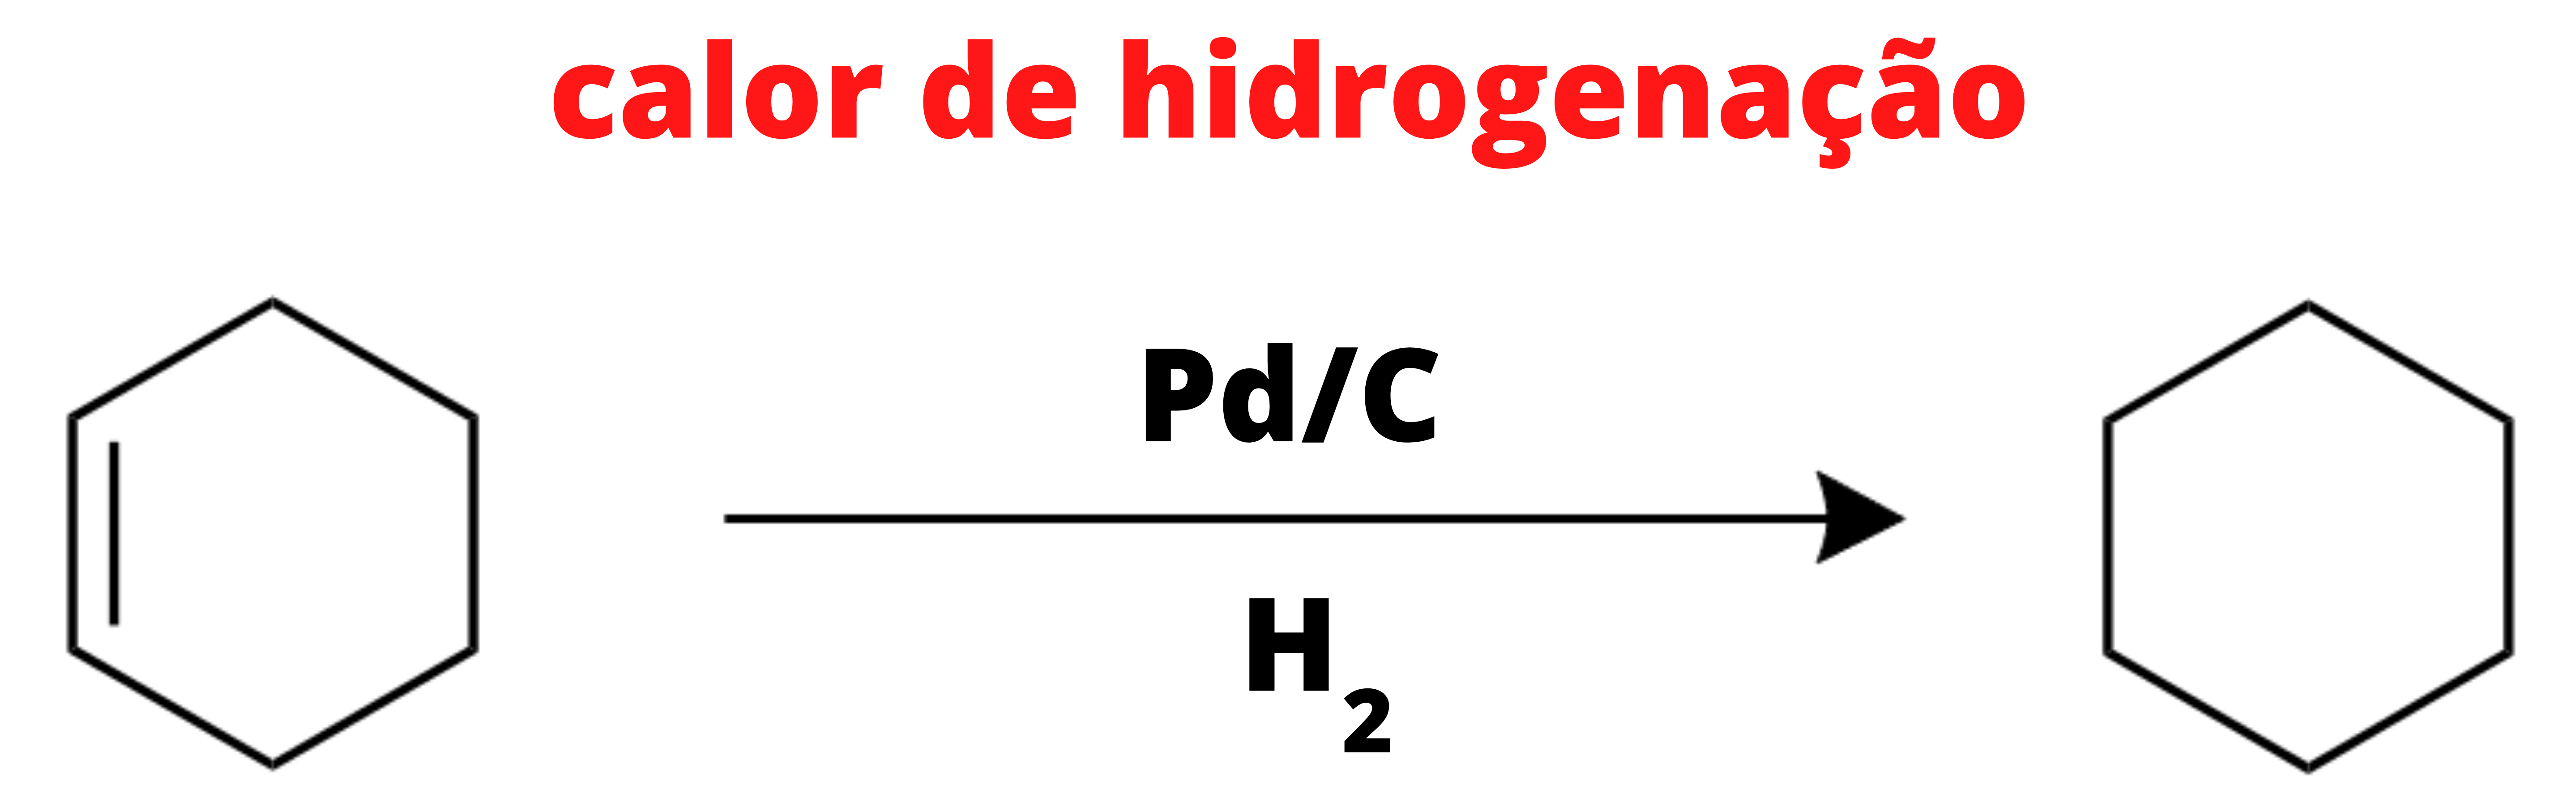
\includegraphics[width=0.5\textwidth]{images/fig1.png}
	\end{center}
	\fonte{Autor(a)}
\end{figure}

Como essa medida é aditiva, se analisarmos o caso do 1,4-cicloexadieno, que possui duas ligações duplas não conjugadas, o calor envolvido no processo será o dobro do que foi observado na situação anterior, isto é, cerca de 56 kcal/mol. No entanto, o isômero conjugado (1,3-cicloexadieno), quando hidrogenado sob as mesmas condições, libera 52,2 kcal/mol (\autoref{fig:2}). A diferença de 3,8 kcal/mol é então chamada de energia de ressonância.

Quando o anel possui três ligações duplas, como na hipótese de um cicloexatrieno, o valor numérico esperado para a entalpia de hidrogenação seria de 85,8 kcal/mol (o triplo do exemplo inicial). Porém, quando essa reação é realizada em condições normais (Pd/C, temperatura ambiente, 1 atm de H$_2$), nada acontece porque o reagente é inerte. Se a pressão for gradualmente aumentada, o cicloexatrieno permanece intacto. Finalmente, submetendo o meio a uma situação drástica (temperatura de 180-220$^\circ$C e 25-30 atm de gás hidrogênio), o reagente hipotético, enfim, gera um cicloexano. Ao medir o calor liberado, o resultado é surpreendente, uma vez que a entalpia obtida é 49,8 kcal/mol, ou seja, 36 kcal/mol abaixo do resultado que era previsto (\autoref{fig:2}). Acontece que o substrato do meio reacional em questão é o benzeno, uma estrutura totalmente conjugada e, por conseguinte, estabilizada pela sobreposição dos orbitais $p$ \autocite{Shaabani2008, Xu2021}. Em função disso, torna-se indispensável a análise comparativa das energias associadas aos orbitais moleculares (\gls{MOs}), uma vez que o caráter covalente da ligação aumenta, e a diferença de energia entre os orbitais de fronteira diminui quando comparamos as espécies aromáticas e seus análogos sem conjugação.

\begin{figure}[htb]
	\caption{\label{fig:2} Calores de hidrogenação relativos aos hidrocarbonetos cíclicos. Em vermelho, são mostradas as energias de estabilização aromática de cada um dos compostos.}
	\begin{center}
		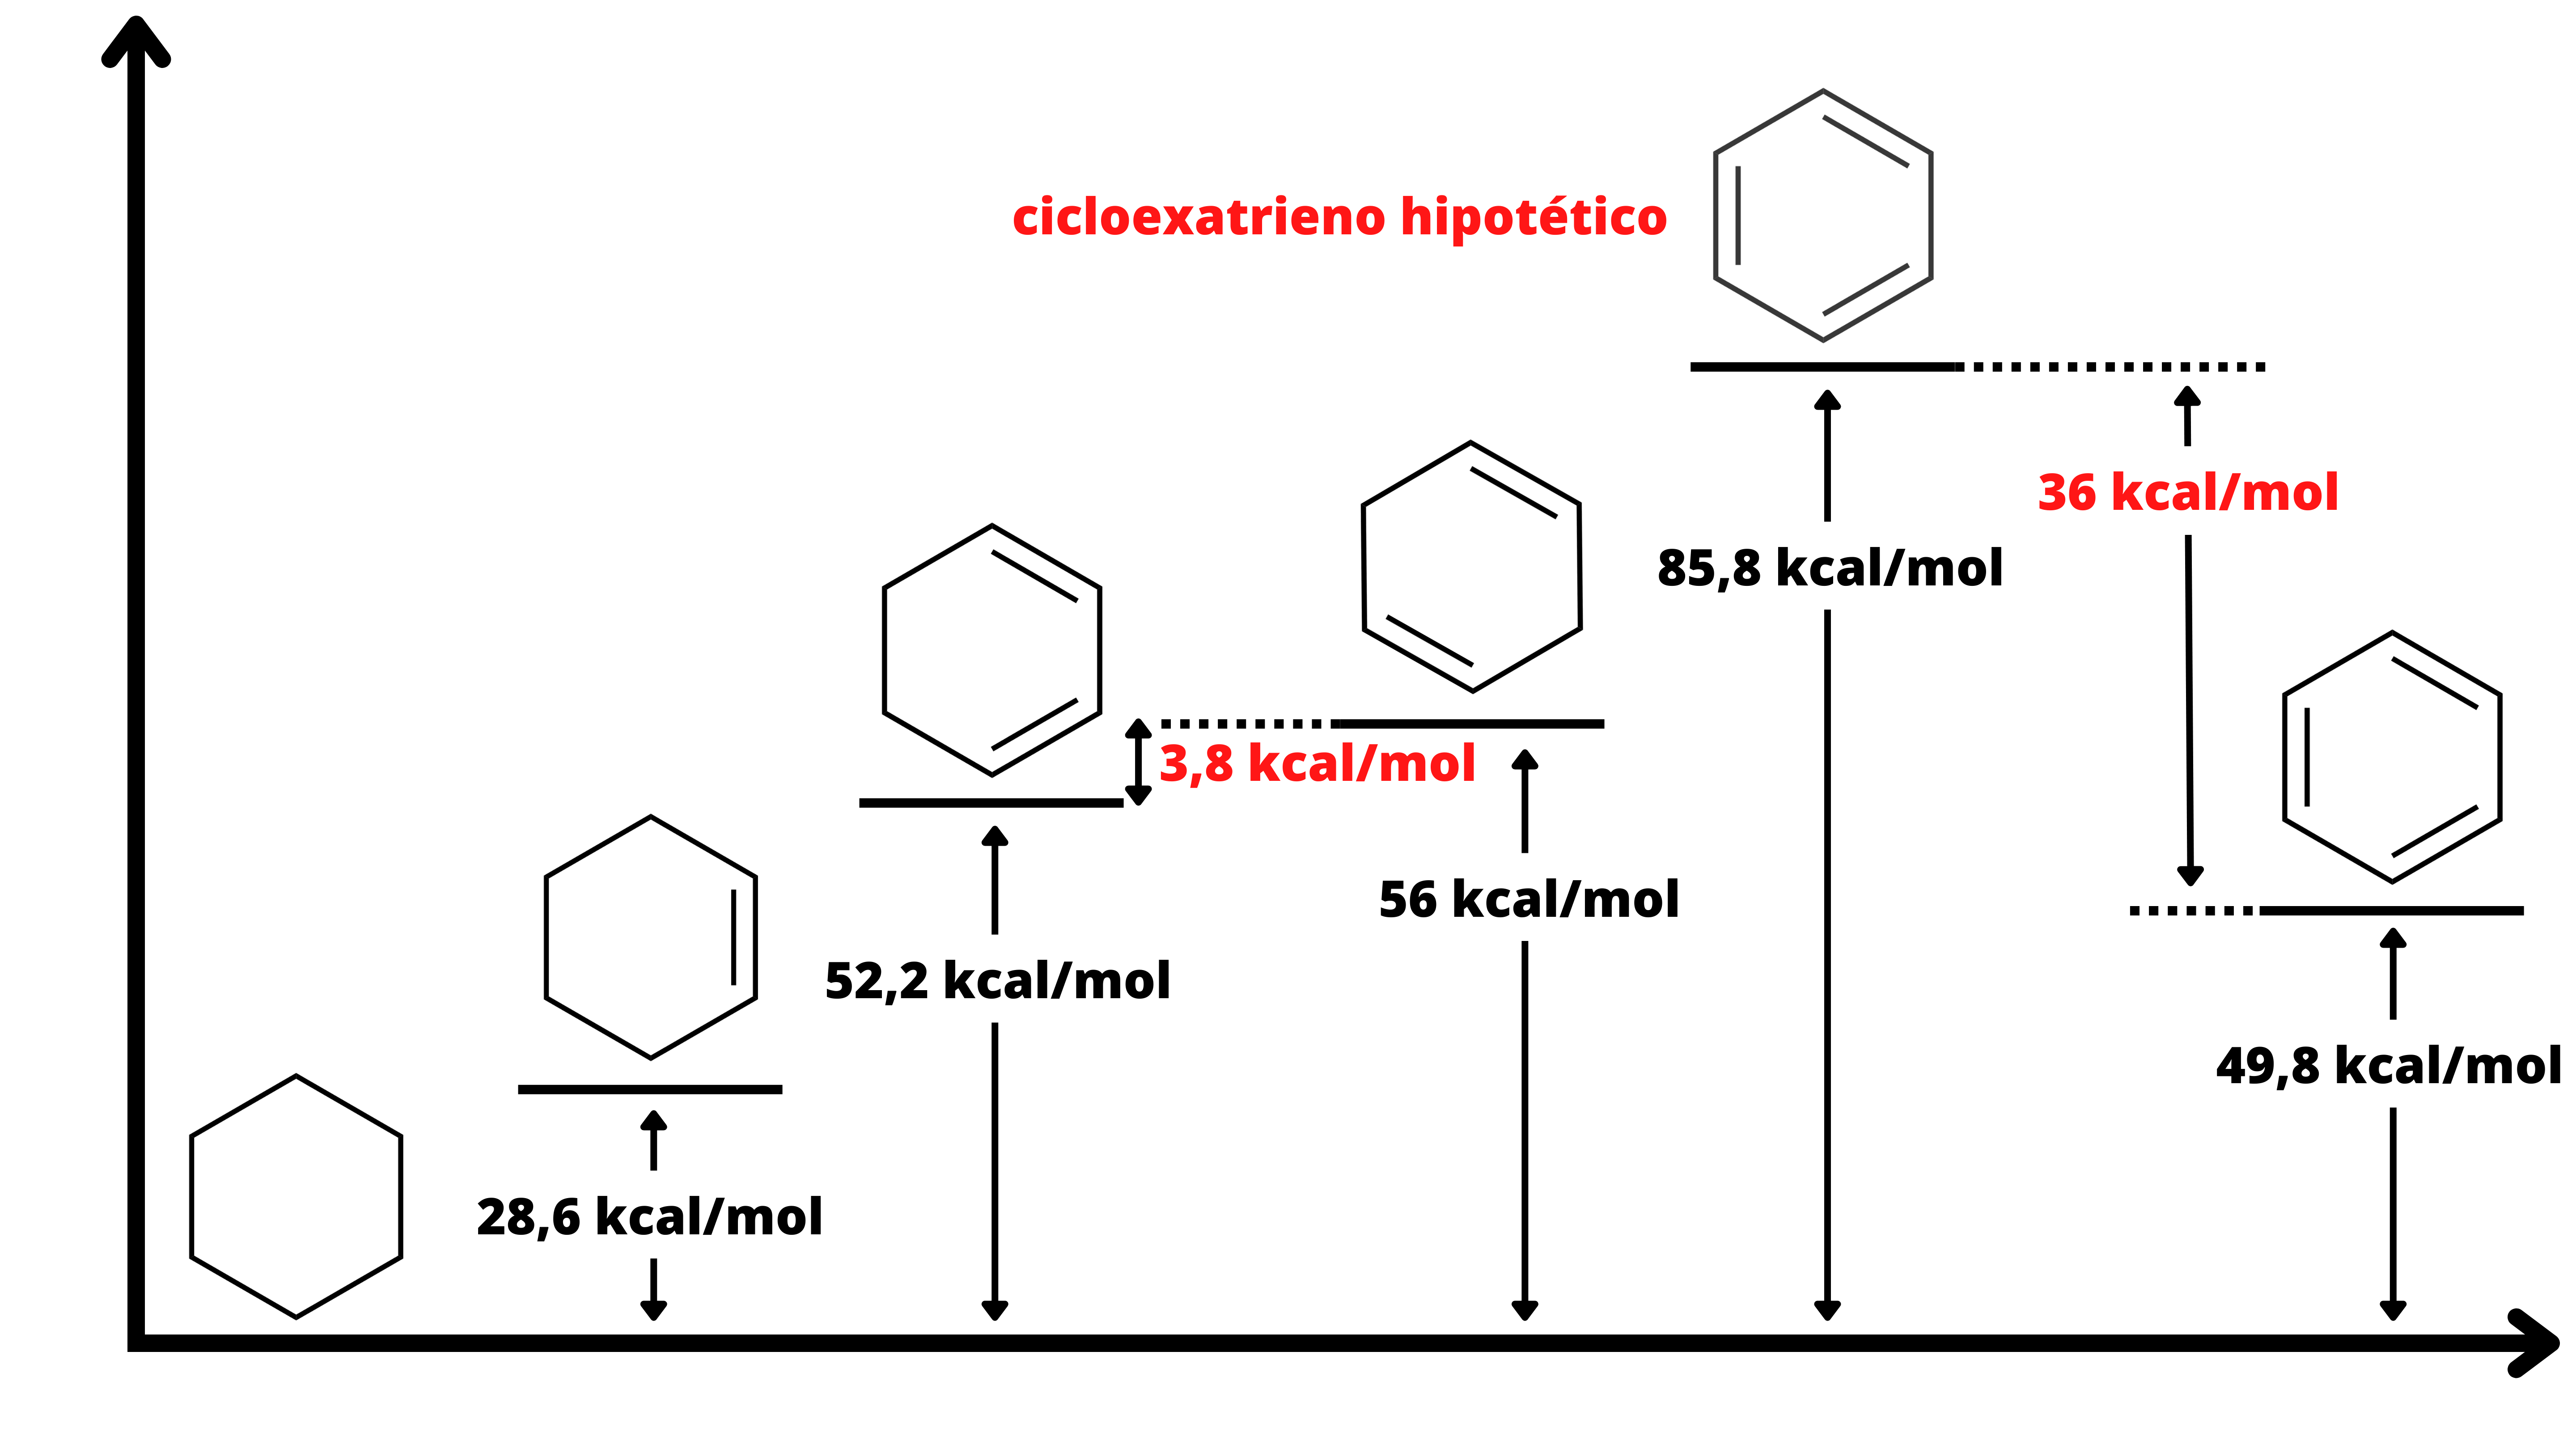
\includegraphics[width=1.0\textwidth]{images/fig2(1).png}
	\end{center}
	\fonte{Autor(a)}
\end{figure}

%% TODO: falar dos orbitais moleculares de fronteira na aromaticidade.

Como o conceito de aromaticidade é multidimensional, um problema recorrente na sua representação é que um dado critério utilizado para classificar hidrocarbonetos, por exemplo, geralmente não pode ser aplicado de maneira consistente, pois encontrar um ponto de referência apropriado é problemático em muitos casos. Por exemplo, os valores de energia de estabilização aromática dependem profundamente dos sistemas de referência em reações virtuais, uma vez que é praticamente impossível deduzir diferenças na aromaticidade de acordo com tendências de reatividade, a menos que sejam consideradas séries de reações estruturalmente similares, a citar, os hidrocarbonetos benzenoides \autocite{Ciesielski2009, Krygowski2014}, do contrário, a intepolação não é verdadeira. Os índices baseados na geometria molecular e alternação dos comprimentos de ligação, tal como o índice de Julg e Françoise \autocite{Julg1967}, também são relativos à escala arbitrária definida previamente, porque são parametrizados de acordo com um único grupo de moléculas de interesse, como os sistemas carbocíclicos derivados do benzeno; e falham miseravelmente para descrever aquilo que está fora dessa escala, a exemplo dos heterociclos aromáticos, que contêm diferenças de eletronegatividade nas ligações entre o heteroátomo e o carbono. Consequências espectroscópicas nos deslocamentos químicos e diferenças topológicas na estrutura eletrônica também podem ser consideradas para classificar um composto orgânico de acordo com a sua aromaticidade. Em 1995, Schleyer \autocite{Schleyer1996} demonstrou que para compostos cíclicos do tipo \ce{(CH)_4 X} existem correlações entre os critérios geométricos, energéticos e magnéticos. Ele escreveu então que:

\begin{citacao}
Tentativas para se racionalizar e quantificar o conceito de aromaticidade devem empregar o maior número de critérios possíveis. Cada categoria de critérios tem suas limitações e ambiguidades\autocite{Schleyer1996}.
\end{citacao}

De acordo com McWeeny, existem também muitas outras noções utilizadas nos laboratórios de química e nas discussões científicas que podem ser classificadas como padrões fundamentais de entendimento (para além da aromaticidade), pois são lançados mão quase que diariamente para compreender processos químicos de maneira intuitiva. De forma mais específica, podem ser mencionados os termos: confôrmero, nucleófilo, eletrófilo, efeito de solvente, ligações de hidrogênio, acidez/basicidade de Lewis. Para analisar isso mais de perto, e de forma comparativa, foi contabilizado o número de trabalhos científicos por dia que citam alguns desses termos. Os dados mostrados na \autoref{fig:3} foram coletados do a partir de uma busca avançada no \href{https://www-periodicos-capes-gov-br.ez46.periodicos.capes.gov.br/index.php?}{\textit{Portal da Capes}}. Através dessa pesquisa, nota-se que o tópico da aromaticidade ocupou o topo das pesquisas durante todo o período analisado (2010-2020), com uma média de 60 artigos publicados por dia em 2020, contra 40 relativos ao tema da análise conformacional.

\begin{figure}[htb]
	\caption{\label{fig:3} Gráfico que relaciona a média de artigos científicos publicados por dia contendo cada um dos termos mostrados na legenda.}
	\begin{center}
		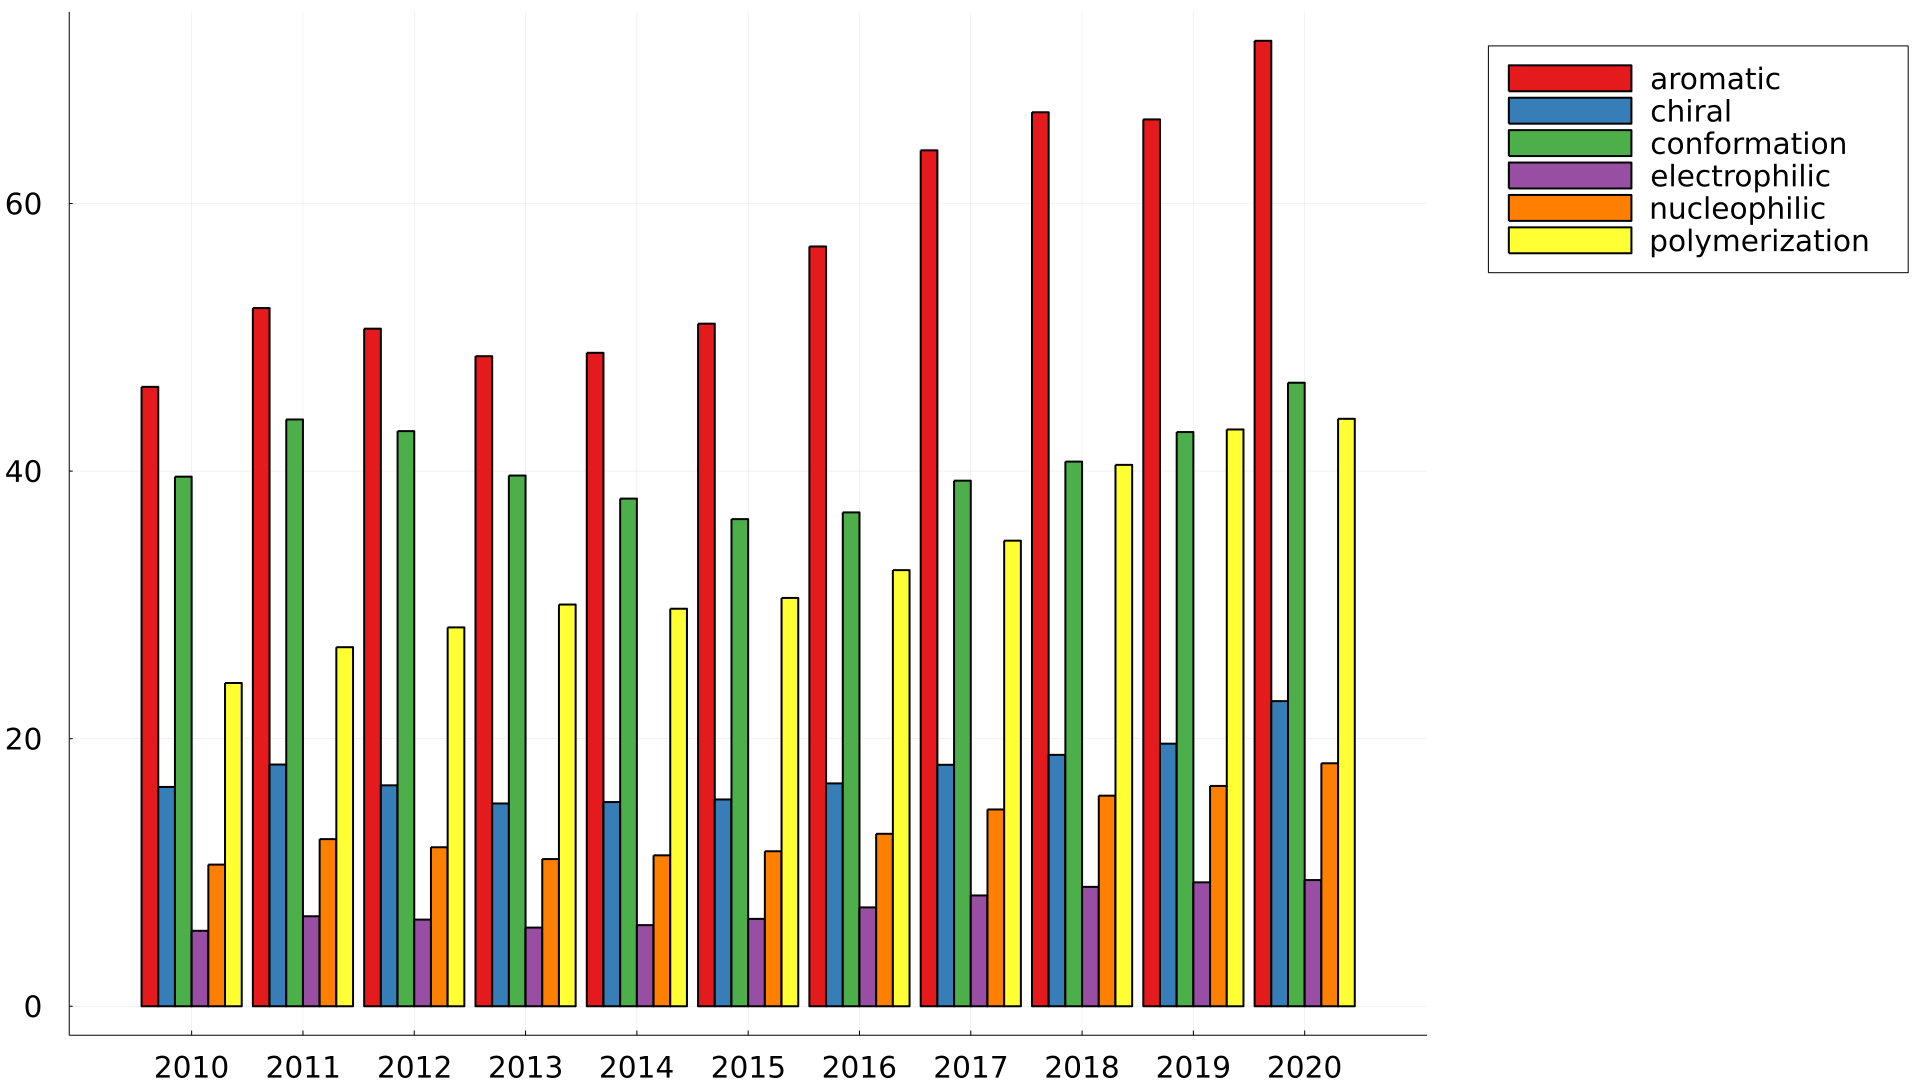
\includegraphics[width=1.0\textwidth]{images/fig3.png}
	\end{center}
	\fonte{Autor(a). Os números são do \href{https://www-periodicos-capes-gov-br.ez46.periodicos.capes.gov.br/index.php?}{\textit{Portal da Capes}}.}
\end{figure}

% Ou seja, a computação gráfica auxilia na manipulação/representação direta dos objetos de estudo químico, sendo eles: átomos, moléculas (leia-se quaisquer agregados atômicos, independentemente da origem de suas interações) ou partes delas. Como esses são elementos de difícil abstração, uma vez que 

% Em tal seguimento, um dos avanços mais importantes é a aplicação da teoria de grafos à notação química e aos sistemas de busca de subestruturas e cálculos de propriedades, como a aromaticidade, que é muito sensível à geometria do sistema $\pi$, pois descreve as moléculas estabilizadas energeticamente pela deslocalização de elétrons móveis em ciclos (geometrias fechadas). Tal temática é extremamente explorada por trabalhos que vem sendo somados desde a primeira citação de Hoffmann na literatura, em 1855. Por exemplo, com uma busca sobre os termos aromático/aromaticidade no \textit{\href{https://scholar.google.com.br/scholar?hl=pt-BR&as_sdt=0\%2C5&as_ylo=2016&as_yhi=2022&q=aromatic&btnG=}{Google Scholar}} no período de 2016 a 2022, foram encontrados mais de 380 trabalhos/dia publicados, sendo a maioria destes na área de Química, uma vez que, entre os compostos carbocíclicos, destacam-se os derivados aromáticos, cuja estabilidade e reatividade dependem do caráter de deslocalização eletrônica. Para tais sistemas, é possível utilizar a equalização dos comprimentos de ligação como principal critério geométrico de análise quantitativa.


Com base nesse conjunto de informações, o presente trabalho visa relacionar as propriedades extraídas das representações moleculares a partir da computação gráfica de forma facilitada e didática através da construção de uma inteface. É sabido que as dificuldades de compreensão por parte dos químicos (em qualquer nível de titularidade) em relação aos conceitos e fenômenos originam-se na forma com que são apresentados \autocite{Cunha2018}. Nesse sentido, a ferramenta proposta poderá ser difundida para uso didático-pedagógico, podendo ser utilizada por discentes e docentes durante as aulas com a intenção de demonstrar os modelos de classificação e a multidimensionalidade da aromaticidade, facilitando o entendimento. O \textit{software} em questão chama-se \textit{Balmy.jl}. A extensão (\textit{.jl}) junto ao nome indica que o mesmo foi produzido na linguagem Julia; e o termo \textit{Balmy}, de origem inglesa, faz alusão ao primeiro critério qualitativo de classificação dos compostos aromáticos: o odor, resgatando a historicidade do conceito de forma criativa.

% Assim, usuário será capaz de calcular os parâmetros geométricos de aromaticidade, um conceito explorado de forma superficial e pouco visual dentro das salas de aula. 

% ----------------------------------------------------------
\chapter{Revisão Bibliográfica}
% ----------------------------------------------------------

Historicamente, as primeiras evidências do uso da terminologia \textit{aromática(o)} remontam ao ano de 1800, mais especificamente à classificação qualitativa\footnote{Importante ressaltar que a noção de \textit{classificação qualitativa} citada pelo trabalho refere-se ao fato de, na época, não se ter conhecimento da estrutura química desses compostos.} de substâncias e óleos essenciais oriundos de produtos naturais através do odor, a exemplo da vanilina e do anetol. Nada obstante, tal ideia caiu em desuso por conduzir, mesmo na época, a associações espúrias como no caso do (-)-mentol (\autoref{fig:4}).

\begin{figure}[htb]
\label{fig:4}
	\caption{Reconhecimento de compostos aromáticos apenas pelo odor.}
	\begin{center}
		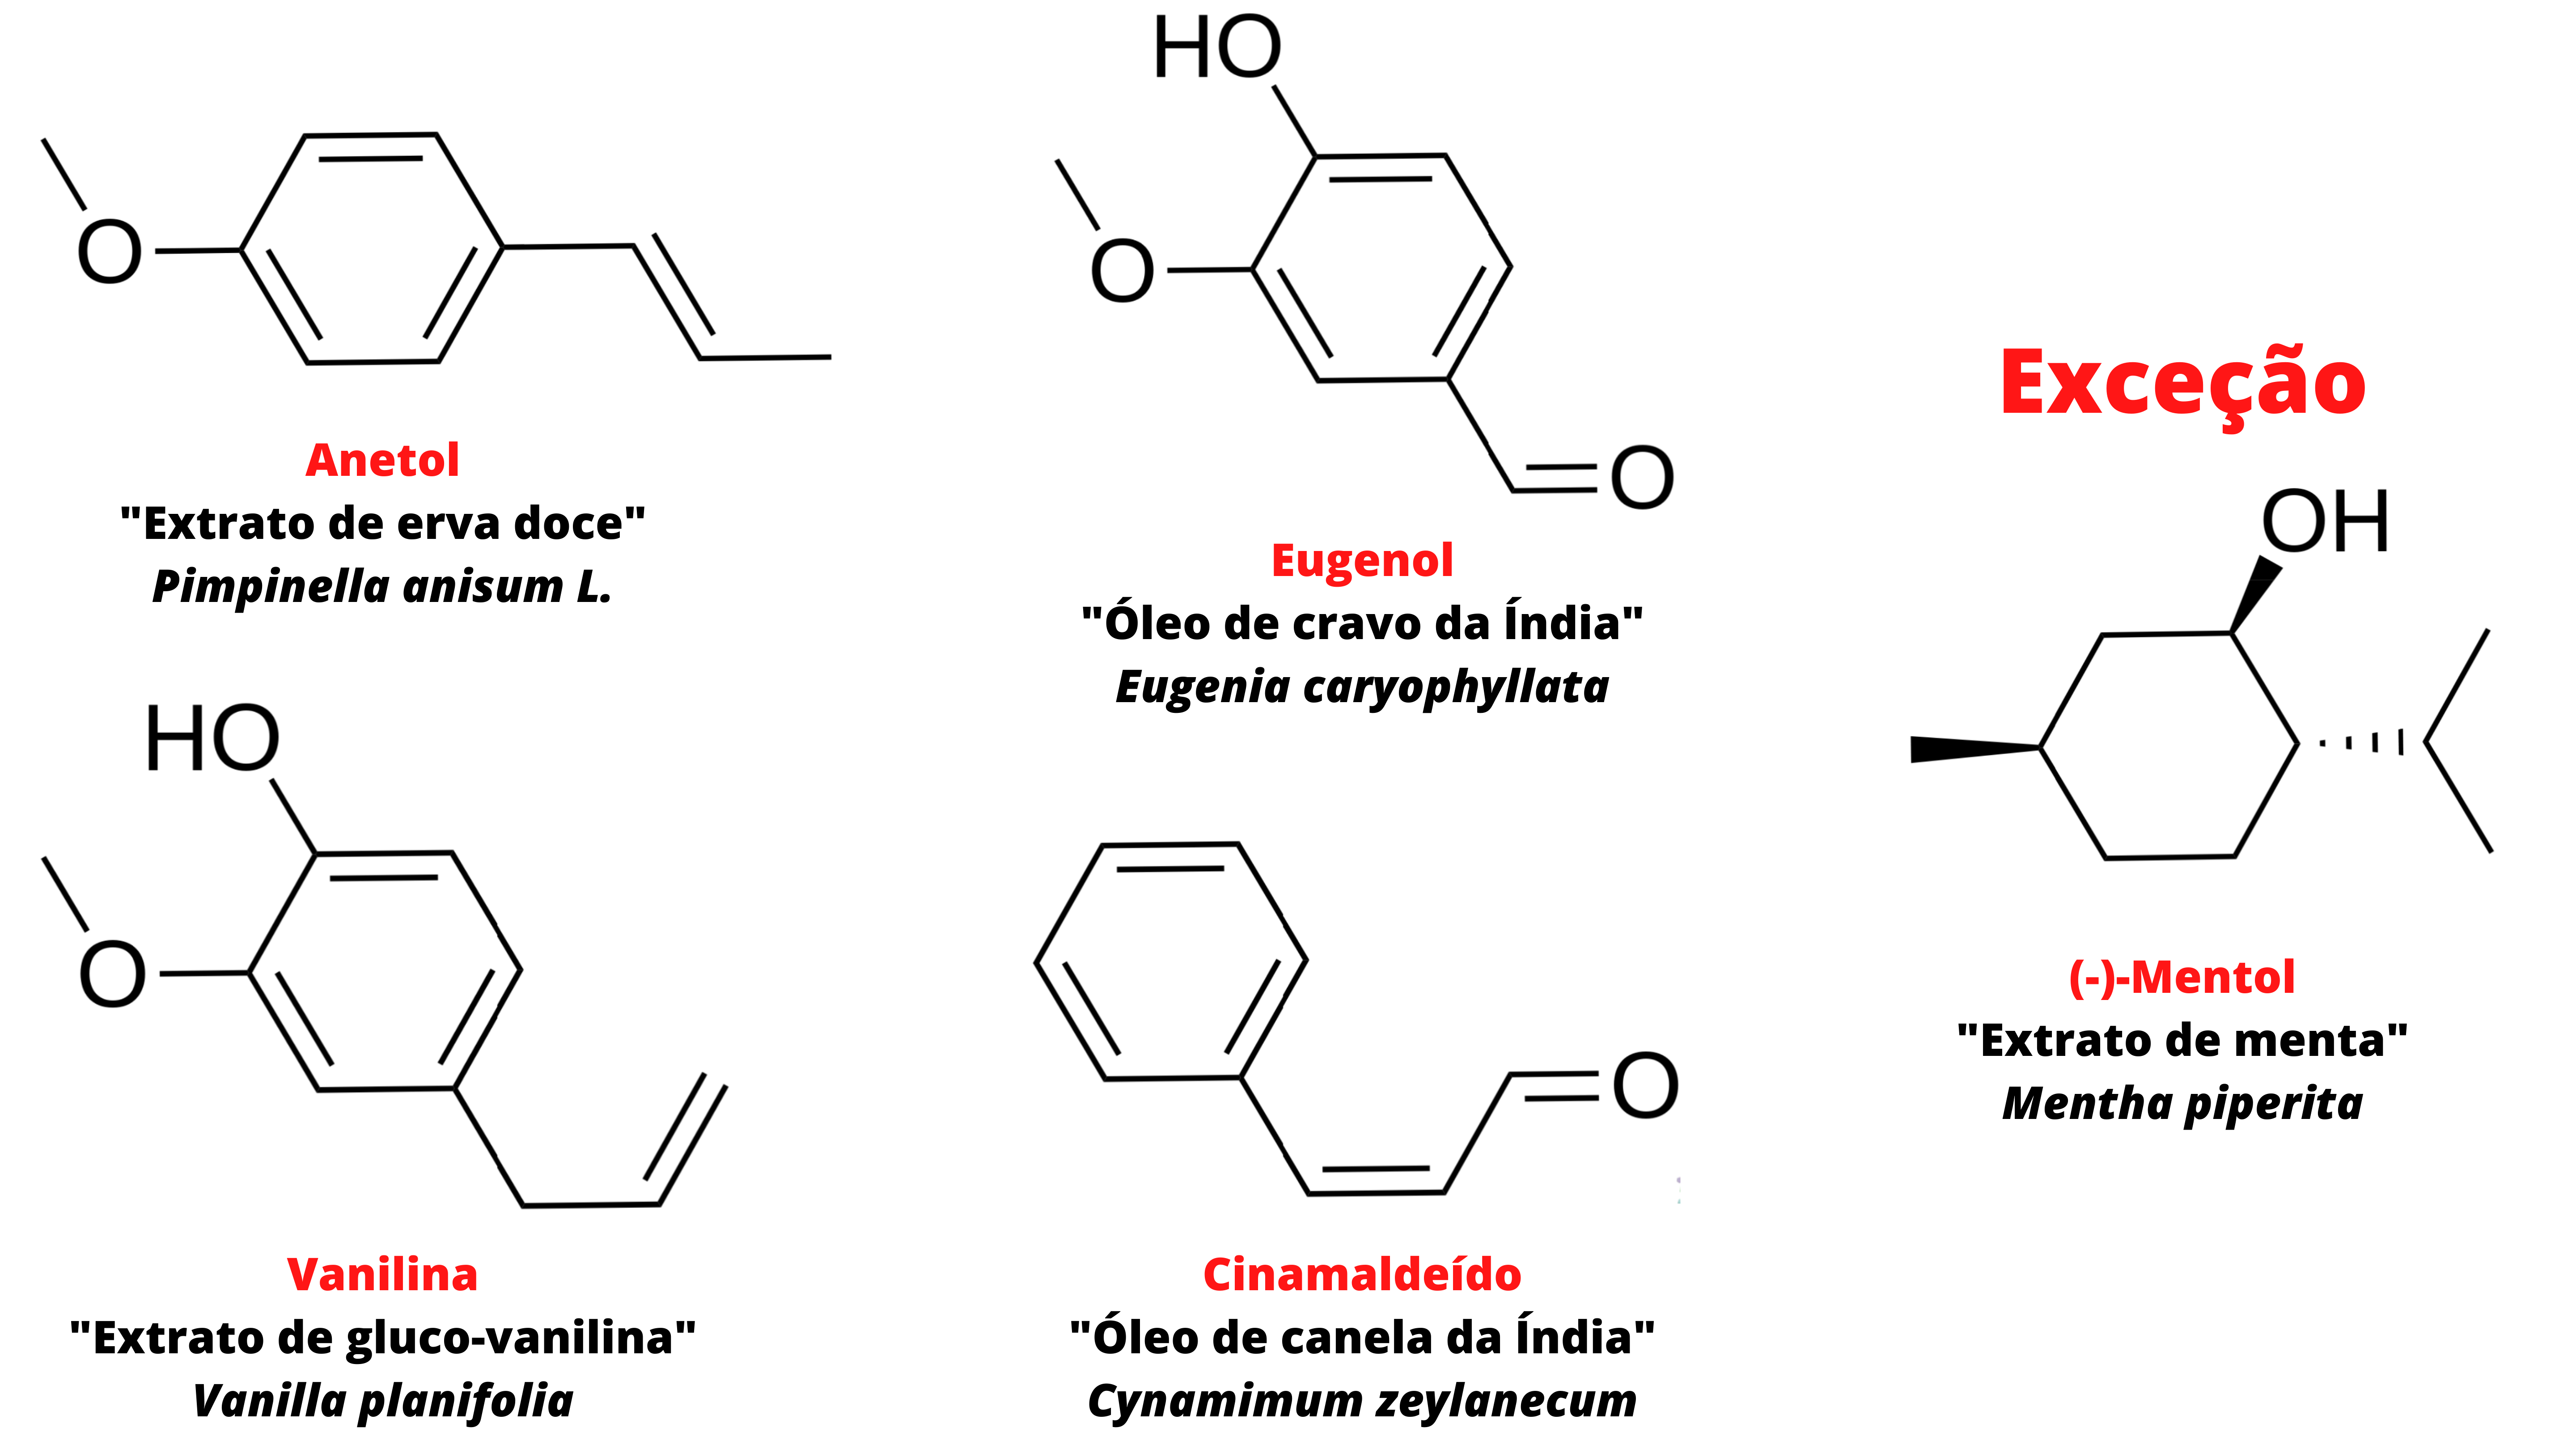
\includegraphics[width=1\textwidth]{images/MOs(1).png}
	\end{center}
	\fonte{Autor(a). Adaptado de Caramori et al. \autocite{Caramori2009}.}
\end{figure}

%% TODO: add the figure of these structures

Décadas depois (1825), Michael Faraday\autocite{Faraday1925, Wilson2012, Martin2015} conseguiu isolar pela primeira vez o benzeno\footnote{O nome do benzeno é derivado do ácido benzoico, descoberto no século XVI. O ácido foi assim designado por ter sido obtido pela destilação seca da goma de benjoim, uma planta nativa da Sumatra, descrita pela primeira ver por Nostradamus em 1555, depois por Aleixo Pedemontanus em 1560 e, em seguida, por Blaise de Vinagère, no ano de 1596}, um hidrocarboneto aromático com alto grau de toxicidade associado\autocite{Solomon1977}. Esse produto foi obtido por fracionamento repetido do fluido obtido durante a compressão do gás petrolífero (o acetileno, usado na iluminação das ruas de Londres, e produzido através da pirólise do óleo de baleia) fornecido através do Sr. Gordon da \href{https://portablegas.co.uk/}{\textit{Portable Gas Company}}. Esse episódio representa um marco extremamente significativo para a construção da ideia de aromaticidade, uma vez que o benzeno é inegavelmente o composto mais famoso dessa classe de moléculas com propriedades decorrentes da deslocalização de elétrons $\pi$\autocite{Faraday1825}. 

Poucos anos depois, em 1834, Eilhard Mitscherlich também realizou a síntese do benzeno, mas agora partindo do ácido benzoico. Esse processo ocorre sob aquecimento na presença de cal virgem (\ce{CaO}), produzindo o benzeno como destilado do meio reacional e calcário (\ce{CaCO_3}) \autoref{fig:4a}. Uma alternativa foi proposta por Mansfield (1845), que isolou o benzeno a partir do alcatrão de hulha sob um procedimento que \textit{a posteriori} foi adaptado à indústria. Apesar da fórmula molecular do benzeno (\ce{C_6H_6}) já ser conhecida em meados do século XIX, restavam muitas dúvidas sobre os aspectos estruturais da molécula, uma vez que a elucidação de estruturas químicas era uma área em defasagem na época. 

\begin{figure}[htb]
	\caption{Síntese de Mitscherlich – benzeno.}
    \label{fig:4a}
	\begin{center}
		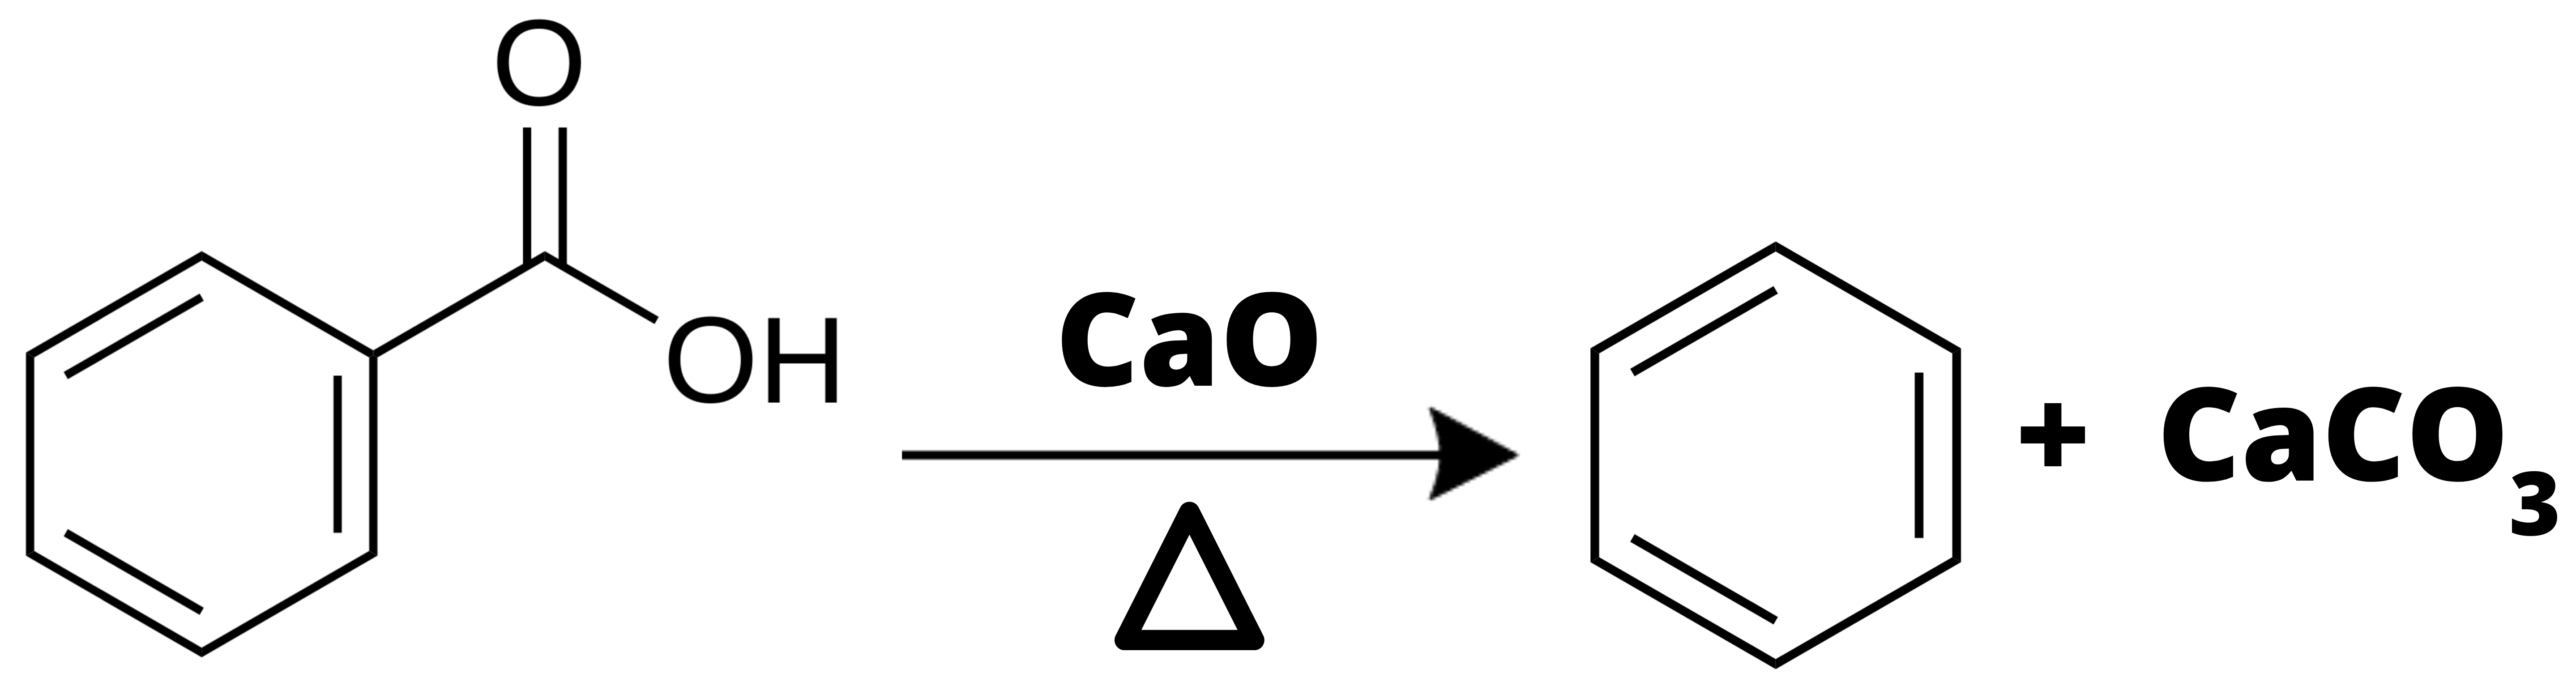
\includegraphics[width=0.65\textwidth]{images/fig2(2).png}
	\end{center}
	\fonte{Autor(a). Adaptado de Caramori et al. \autocite{Caramori2009}.}
\end{figure}

Foi então nos anos 1860 que químicos como Loschimidt (1861), Laderburg (1869), Claus (1866) e Dewar (1866) (\autoref{fig:5}), começaram a intencionar hipóteses sobre a estrutura do benzeno, até chegar, em 1865, na proposta de Kekulé, que se assemelha mais ao que seria a real representação estrutural do composto, fato que só foi devidamente reconhecido décadas mais tarde (1890) e comprovado em 1929\autocite{Lonsdale1929}, com a obtenção da primeira estrutura por difração de raios-X de um derivado, o hexametilbenzeno.

\begin{figure}[htb]
	\caption{Propostas para a estrutura do benzeno.}
    \label{fig:5}
	\begin{center}
		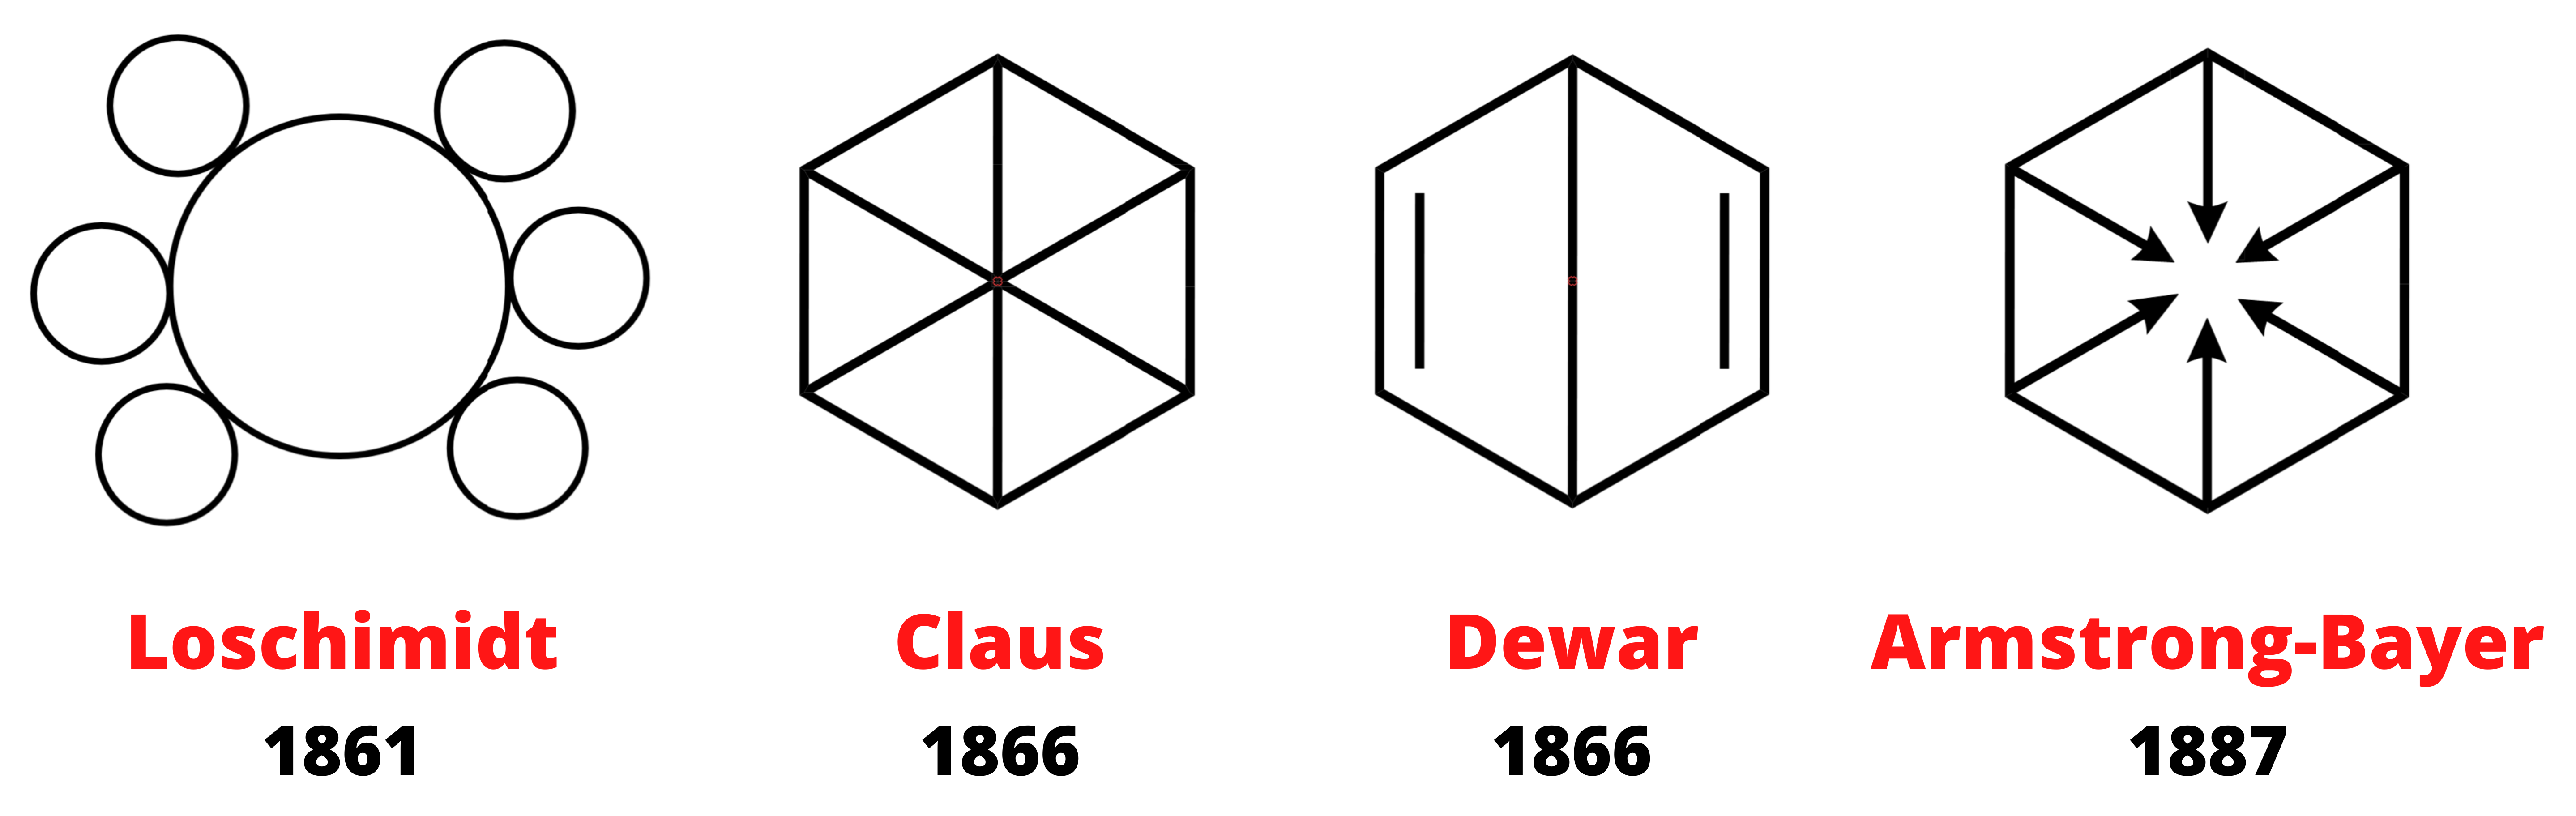
\includegraphics[width=0.65\textwidth]{images/8(1).png}
	\end{center}
	\fonte{Autor(a). Adaptado de Caramori et al. \autocite{Caramori2009}.}
\end{figure}

Com a virada do século XIX para o XX, passou-se a ganhar entendimento da inexistência de
um equilíbrio formal entre as formas isoláveis do benzeno, mas sim das estruturas canônicas de ressonância que perfazem um híbrido com elétrons móveis através de um efeito isomérico chamado mesomeria \autocite{Murrell1956, INGOLD1934, Oudar1975} (\autoref{fig:7}). 

\begin{figure}[htb]
	\caption{Estruturas de ressonância do benzeno.}
    \label{fig:7}
	\begin{center}
		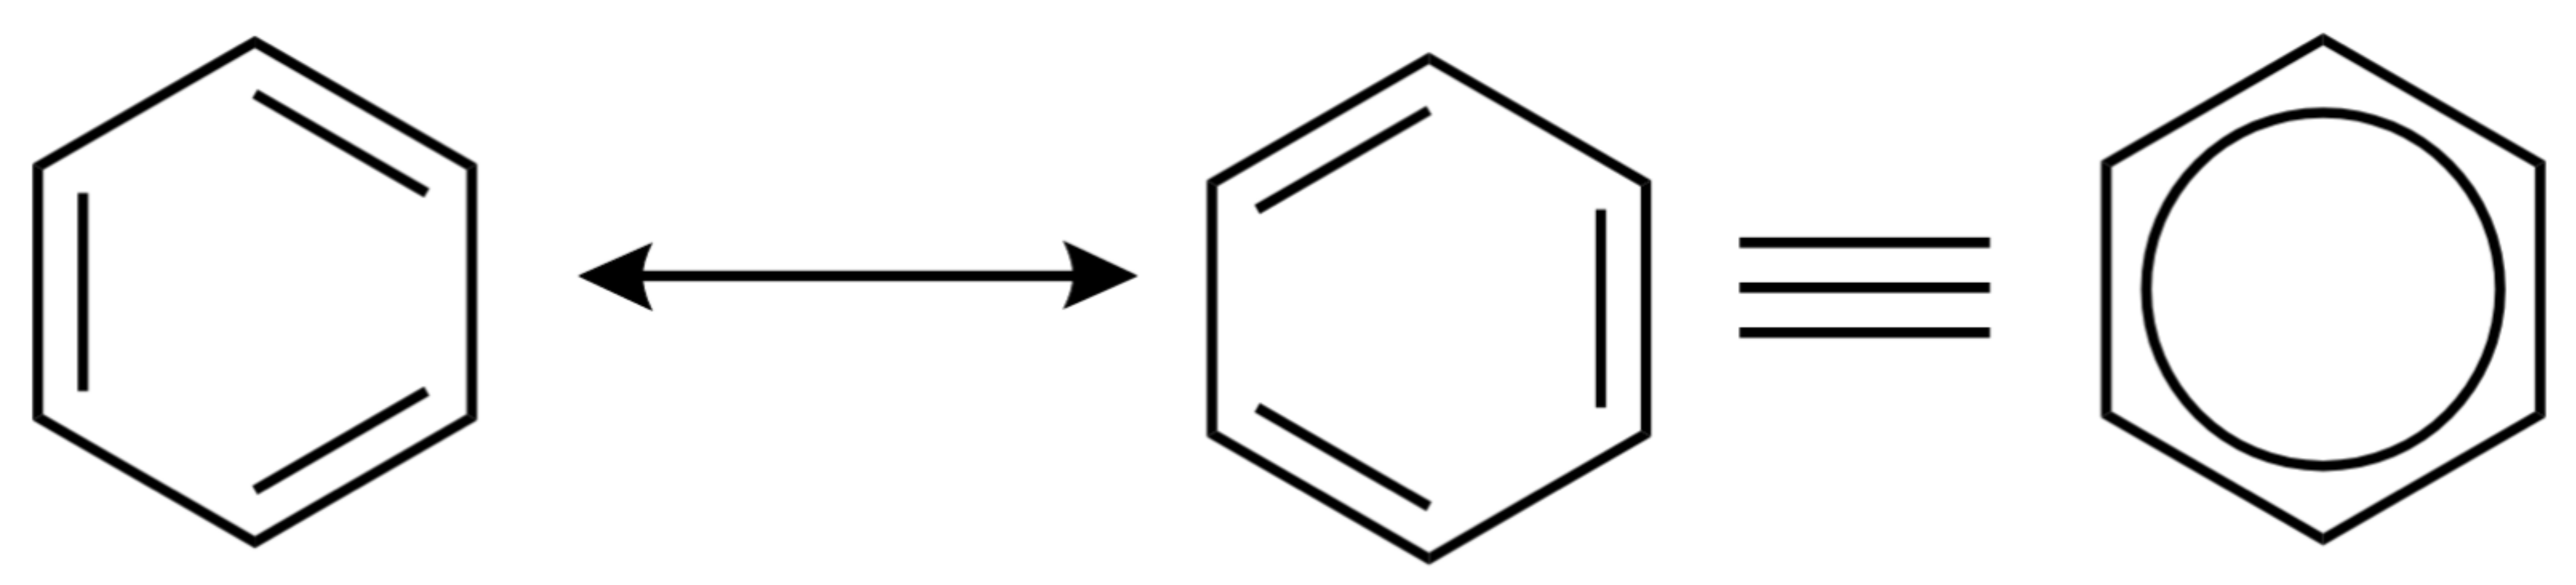
\includegraphics[width=0.6\textwidth]{images/7.png}
	\end{center}
	\fonte{Autor(a). Adaptado de Caramori et al. \autocite{Caramori2009}}
\end{figure}

Ou seja, a cada geração de químicos que estudavam a estrutura do benzeno e seus análogos, tanto para fins sintéticos, quanto para fins práticos, de aplicações, o conceito de \textbf{\textit{aromaticidade}} aparecia de forma elusiva e abstrata, mas sem uma conceituação descritiva e quantitativa. Desse modo, as definições prosseguiram das observações experimentais associadas aos resultados termoquímicos, como os calores de hidrogenação, por exemplo, uma vez que os compostos aromáticos (sejam eles benzenoides ou não) são mais estáveis e possuem geometrias mais planares do que análogos saturados. Mais recentemente, a química computacional também tornou-se útil para realizar essas análises \autocite{Jiao1997}, utilizando métodos teóricos (otimização de geometrias, cálculo de orbitais moleculares, simulações espectroscópicas) para investigar esse tipo de propriedade na mais diversa variedade de sistema, como nanotubos \autocite{Matsuo2003}, por exemplo. Sumariamente, é correto afirmar que um conceito fenomenológico abstrato (no caso, a aromaticidade) pode ser interpretado de forma multidimensional.

Os compostos insaturados aromáticos também possuem propriedades aditivas inerentes aos átomos e ligações que os constituem, como a exaltação da susceptibilidade magnética\autocite{Schleyer1996, Schleyer2001, Schleyer2014}. Segundo Pascal (1910) no artigo intitulado \textit{Magnetochemical researches}\autocite{pascal1910magnetochemical}, a mobilidade eletrônica em estruturas cujas ligações duplas são alternadas torna-as diamagnéticas, isto é, não possuem magnetização a campo zero e apresentam uma magnetização contrária quando um campo é aplicado. Por isso, os compostos aromáticos são capazes de induzir campos magnéticos significativos a ponto de interferir nas frequências de ressonância de átomos ligados ao anel aromático. Neste caso, são conhecidos os efeitos de proteção e desproteção de núcleos provocados pelas correntes de anel.

\begin{figure}[htb]
	\caption{\label{fig:2} Correntes de anel e linhas de força induzidas no benzeno}
	\begin{center}
		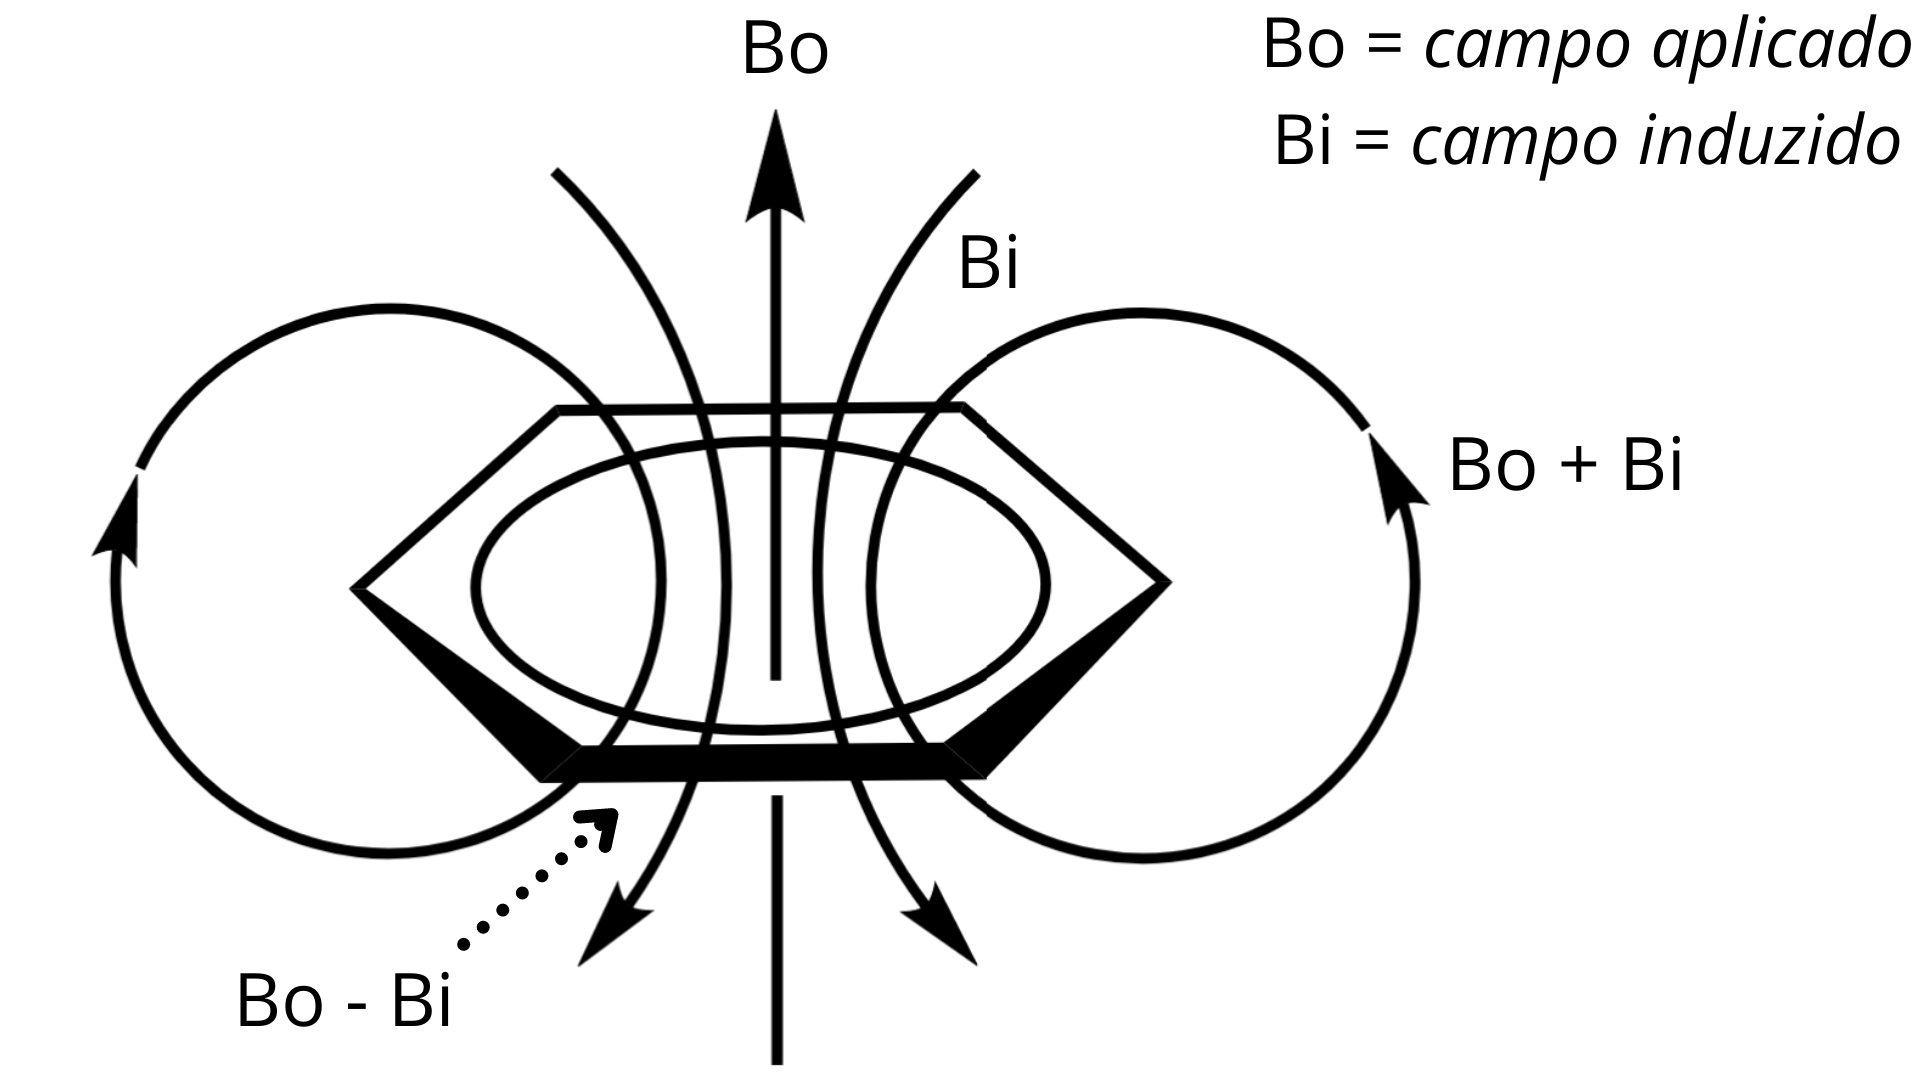
\includegraphics[width=0.60\textwidth]{images/magneticoPascal.png}
	\end{center}
	\fonte{Autor(a). Adaptado de Caramori et al. \autocite{Caramori2009}}
\end{figure}

Foi então no ano de 1931, quando a fundamentação estrutural da aromaticidade se tornava mais sólida, que surgiu uma das primeiras regras de classificação de moléculas aromáticas desenvolvida por Erich Hueckel\autocite{Hckel1931}. Ele baseou-se na ideia de que as estruturas eletrônicas que requerem circuitos fechados de elétron móveis são extremamente sensíveis a alterações na simetria de suas funções de onda em decorrência do número de elétrons \autocite{Hckel1931, Schleyer1996, Schleyer2001}. Utilizando a teoria dos orbitais moleculares, ele elucidou muitos pontos sobre as propriedades eletrônicas de compostos orgânicos, o que o permitiu demonstrar que hidrocarbonetos cíclicos com ($4n+2$) elétrons $\pi$ (sendo $n$ um número inteiro) possuem um incremento da estabilidade energética. Hueckel\autocite{Hckel1931, Brogli1972} justificou este efeito através da distribuição eletrônica dos compostos aromáticos, uma vez que, para ele, a razão do abaixamento da energia dos compostos aromáticos devia-se à ausência de elétrons desemparelhados.

Tal abordagem tem, no entanto, suas excepcionalidades, a exemplo dos [10]anulenos, que possuem o número adequado de elétrons $\pi$, mas não as demais propriedades associadas à aromaticidade (estabilidade, reatividade, propriedades magnéticas típicas). Essa distorção é causada por fatores topológicos e efeitos estereoeletrônicos observados nesses compostos, pois os hidrogênios internos das estruturas dos [10]anulenos afetam boa conjugação do sistema $\pi$ \autocite{Caramori2006}. 

Com a intenção de ampliar a regra de Hueckel para hidrocarbonetos policíclicos aromáticos, foi criado um modelo inspirado no trabalho de Armit e Robinson, que definiram o um sexteto $\pi$, que compreende seis elétrons $\pi$ num único anel de benzeno, separados por anéis adjacentes com ligações simples CC. A regra de Clar diz que a estrutura de ressonância com o maior número de sextetos $\pi$ aromáticos disjuntos é a mais importante para a caracterização das propriedades dos hidrocarbonetos policíclicos aromáticos. Múltiplas evidências experimentais e teóricas provam que as propriedades físico-químicas dos hidrocarbonetos benzenoides são bem explicados pela regra de Clar \autocite{Sola2013}. 

Do ponto de vista experimental, o primeiro sucesso do modelo foi explicar a razão pela qual o \textit{benzo[qr]nafto[2,1,8,7-fghi]pentaceno}
reagiu prontamente com anidrido maleico, enquanto seu isômero \textit{tribenzo[fg,ij,rst]pentafeno} não foi reativo \autoref{fig:exampledd}. Comparando esses dois produtos, torna-se evidente que a estrutura do \textit{tribenzo[fg,ij,rst]pentafeno} é quimicamente inerte, pois contém 5 benzenoides, enquanto que a estrutura do \textit{benzo[qr]nafto[2,1,8,7-fghi]pentaceno} pode agir como um dieno em uma reação Diels-Alder \autocite{Clar1958}.

\begin{figure}[htb]
	\caption{\label{fig:exampledd}Representação das estruturas (\textbf{a}) benzo[qr]nafto[2,1,8,7-fghi]pentaceno e (\textbf{b}) tribenzo[fg,ij,rst]pentafeno, onde (\textbf{b}) é a estrutura de Clar.}
	\begin{center}
		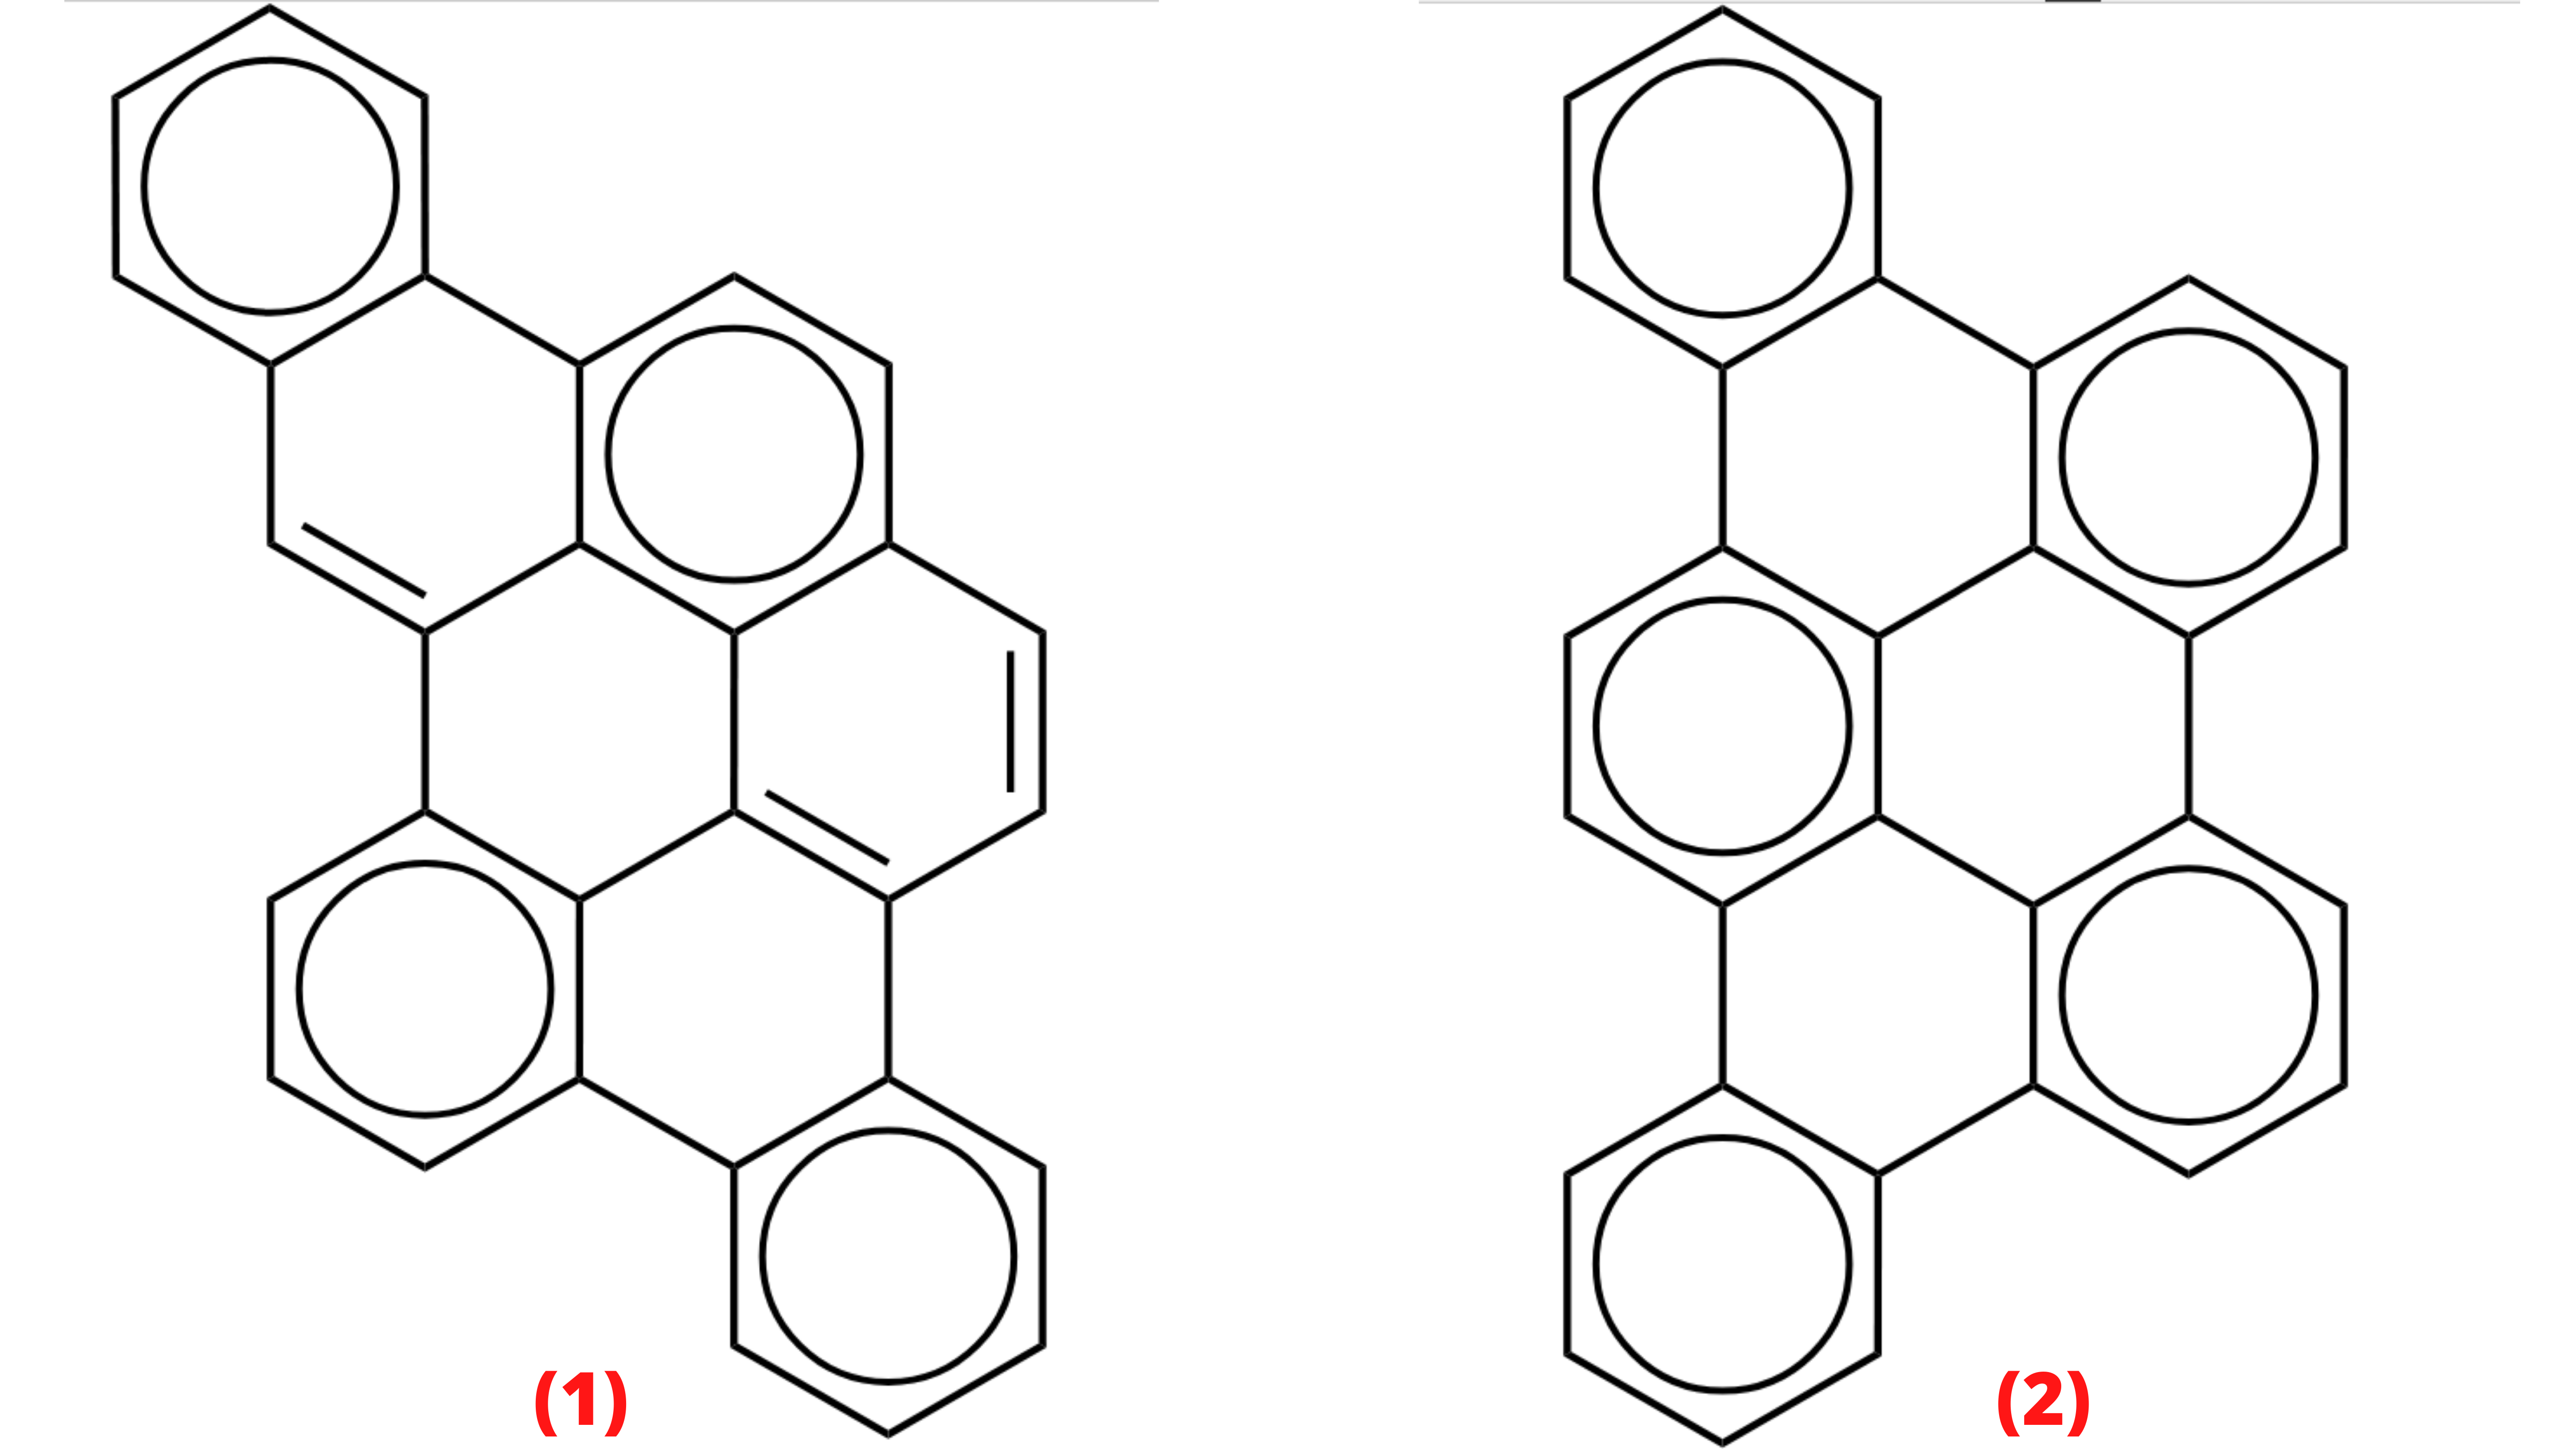
\includegraphics[width=0.75\textwidth]{images/14.png}
	\end{center}
	\fonte{Autor(a).}
\end{figure}

Ou seja, surgiram algumas estratégias experimentais para a determinação das energias de ressonância, que justificam o aumento da estabilidade dos compostos aromáticos. Pauling (1933) \autocite{Pauling1933, Pauling1936} e Kistiakowsky (1936) calcularam a energia de ressonância do benzeno (e de alguns compostos benzenoides) baseando-se nos calores de hidrogenação ($\Delta H^{\circ}_{\textit{hidrogenação}}$) de algumas reações selecionadas. Eles encontraram valores em torno de 36 kcal/mol para o benzeno, o que serviu para comparar com os parâmetros já conhecidos para alcenos não conjugados e assim aprofundar o estudo físico-químico da aromaticidade. Dessa forma, com o avanço da química quântica e dos métodos teóricos de análise dos arranjos atômicos no século XX, evoluíram também os critérios para se avaliar se os compostos podem ser classificados como:

\begin{enumerate}
    \item \textit{aromáticos} (estabilizados por ressonância de elétrons);
    \item \textit{não-aromáticos} (não sofrem efeito mesomérico);
    \item \textit{antiaromáticos} (desestabilizados por efeitos geométricos, torcionais e estereoeletrônicos); quais sejam, de origem geométrica, magnética e energética. 
\end{enumerate}

\section{Critérios Geométricos}

A geometria molecular é um fator primordial para determinar a aromaticidade quantitativamente, uma vez que a alternação dos comprimentos de ligação devido à deslocalização cíclica de elétrons tem sido considerada como um critério fundamental de tal propriedade. Esse fato não se associa somente aos elétrons $\pi$, mas também com elétrons $\sigma$ ou pode ainda apresentar um caráter misto \autocite{Evans1938, Evans1938a, Evans1939}.

Nesse sentido, um parâmetro geométrico só faz-se confiável quando a estrutura analisada é obtida de forma acurada, seja experimentalmente, através de técnicas como difração de raios-X\footnote{Aqui podem ser citadas outras técnicas, a exemplo da difração de elétrons em fase gás, espectroscopia de microondas e difração de nêutrons, mas a difração de raios-X tem sido a mais empregada na determinação de estruturas moleculares, uma vez que os outros métodos são mais restritos por se aplicarem somente a moléculas mais simples e com alta simetria.}, ou de maneira teórica, por meio de cálculos \textit{ab initio} e \gls{DFT} (onde as geometrias são totalmente dependentes do nível de teoria empregado). Isso se torna tão mais importante quanto maior é o interesse em visualizar/analisar pequenas diferenças de aromaticidade.

Os critérios geométricos são aplicados não somente à molécula inteira, como nos outros critérios, mas também podem ser utilizados para estudar fragmentos de sistemas $\pi$-eletrônicos cíclicos ou não. Os indicadores \gls{NICS} pode, por sua vez, ser aplicados aos anéis individualmente (dependendo do tamanho do ciclo em questão). Em quase todos os casos considerados, os índices geométricos descrevem o grau de elétrons-$\pi$ ou deslocalização de ligações duplas. A natureza da equalização dos comprimentos de ligação dupla é amplamente investigada, mas aqui, aceitamos o pressuposto de que ela é advinda da deslocalização eletrônica.

Ou seja, os índices geométricos servem para três propósitos centrais:

\begin{enumerate}
    \item estimar o caráter aromático de uma dada molécula em comparação a outras;
    \item testar novas características numéricas por análises estatísticas de similaridade com outros índices;
    \item estudar as mudanças na aromaticidade devido às perturbações intra- ou intermoleculares.
\end{enumerate}

No presente trabalho, daremos enfoque ao estudo dos critérios de classificação e quantificação baseados na equalização dos comprimentos de ligação, tratando a aromaticidade do ponto de vista estrutural. Além disso, também serão exploradas análises com base na teoria dos orbitais moleculares de Hueckel.

\subsection{O índice de Julg Aj (1967)}

A primeira abordagem quantitativa da definição de aromaticidade foi desenvolvida por Julg et al. \autocite{Julg1967, Bergmann1971}, baseado na ideia de que a alternação dos comprimentos de ligação caracteriza o decréscimo da aromaticidade. Foi construída uma função normalizada da variância dos comprimentos de ligação CC no perímetro de sistemas carbocíclicos $\pi$-eletrônicos.

\begin{figure}[htb]
    \vspace{2\baselineskip}
\begin{equation}
    \label{eq:1}
    A_j = 1 - \frac{225}{\tikzmarknode{numberOfBonds}{\highlight{blue}{$n$}}} \sum^n_{i=1} \bigg{(}1 - \frac{\tikzmarknode{bondLengths}{\highlight{red}{$R_i$}}}{\tikzmarknode{bondAverage}{\highlight{red}{$R_{av}$}}} \bigg{)}^2
\end{equation}
\begin{tikzpicture}[overlay,remember picture,>=stealth,nodes={align=left,inner ysep=1pt},<-]
    \path (numberOfBonds.south) ++ (-1,-2em) node[anchor=north east,color=blue!67] (scalep){\textit{número de ligações}};
    \draw [color=blue!87](numberOfBonds.south) |- ([xshift=-2.5em,color=blue]scalep.north west);
    
    \path (bondLengths.north) ++ (1,2em) node[anchor=south west,color=red!67] (scalep){\textit{comprimento de ligação}};
    \draw [color=red!87](bondLengths.north) |- ([xshift=1.0em,color=red]scalep.south east);
    
    \path (bondAverage.south) ++ (1,-2em) node[anchor=north west,color=red!67] (scalep){\textit{$\displaystyle R_{av} = \frac{\displaystyle \sum_{i=1}^{n} R_i}{\displaystyle n}$}};
    \draw [color=red!87](bondAverage.south) |- ([xshift=4.3em,color=red]scalep.north east);
\end{tikzpicture}
    \vspace{4\baselineskip}
\end{figure}

Na \autoref{eq:1}, a constante 225 resulta da condição de normalização, onde $A_j = 0$ no caso na estrutura do benzeno de Kekulé (cujos comprimentos de ligação seriam diferentes). Para qualquer sistema que possui todas as ligações do mesmo comprimento, o valor de $A_j = 1$. A limitação do método é que este só se aplica a sistemas carbocíclicos, tornando-se inviável sua aplicação a sistemas aromáticos que contenham heteroátomos, pois exclui contribuições que são devidas às interações entre heteroátomos e carbonos levando, portanto, a uma interpretação errônea da aromaticidade.

\begin{figure}[htb]
	\caption{\label{fig:radialenos} Exemplos de radialenos.}
	\begin{center}
		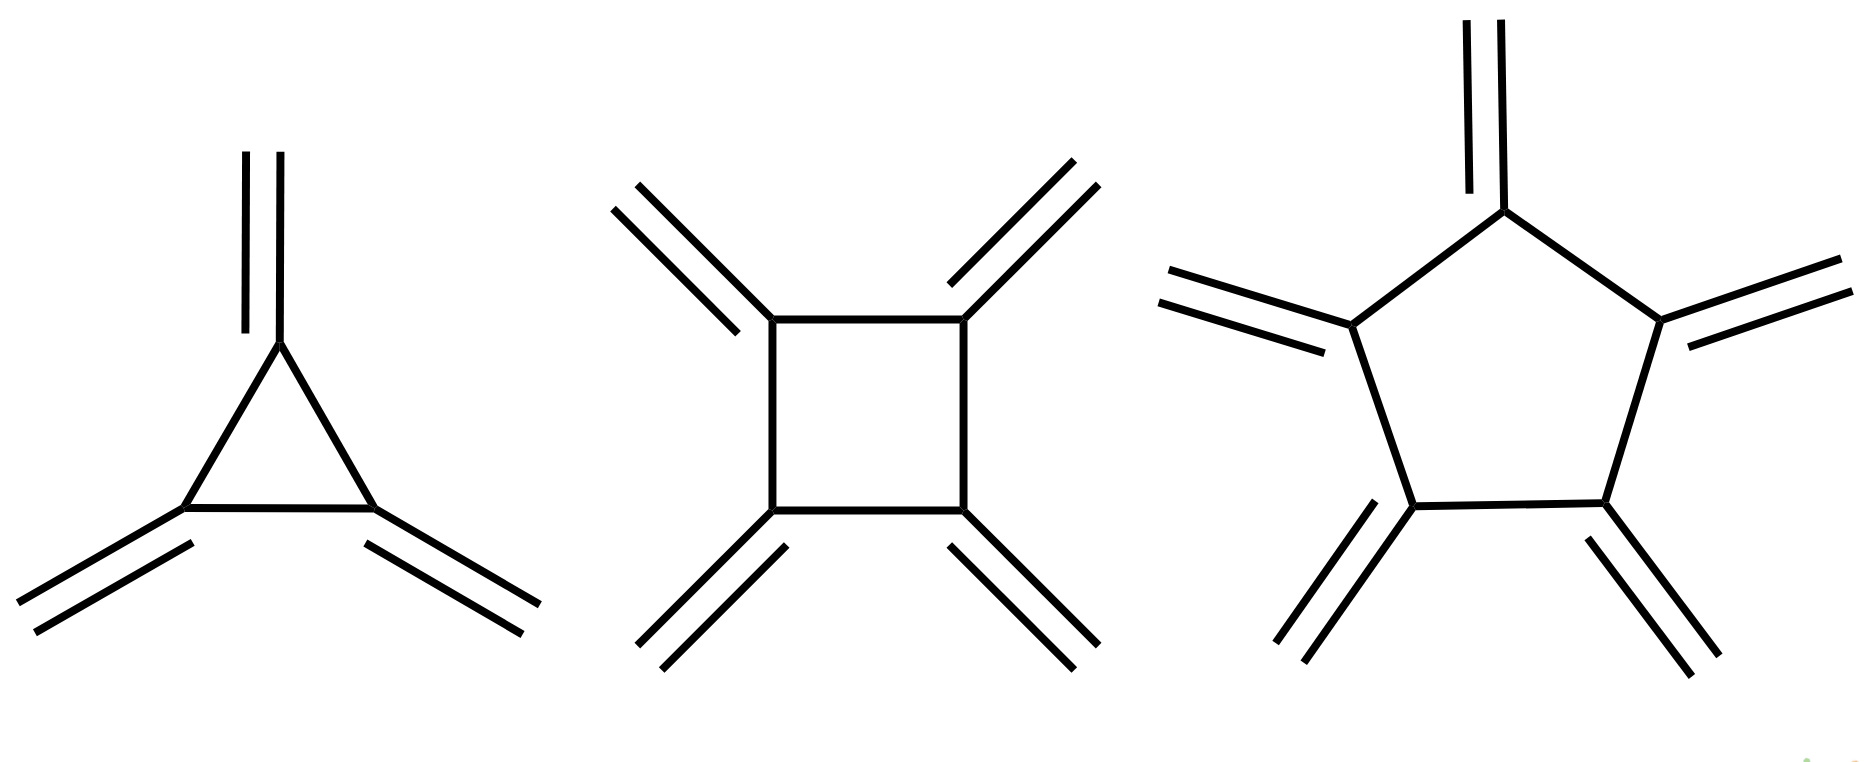
\includegraphics[width=0.70\textwidth]{images/Screenshot from 2022-07-13 13-24-27.png}
	\end{center}
	\fonte{Autor(a).}
\end{figure}

Outro problema intrínseco ao método foi observado ao avaliar a aromaticidade para sistemas de elétrons $\pi$ contendo todas as ligações com o mesmo comprimento, a exemplo dos radialenos (antiaromáticos) \autoref{fig:radialenos}, que apresentam todas as ligações CC alongadas ($1.53$ \AA) em comparação ao benzeno ($1.40$ \AA), mas apesar disso apresenta $A_j = 1$, o que é evidentemente incorreto, conforme demonstrado pelo índice \gls{HOMA} e pelo NICS.

\subsection{Análise das ordens de ligação}

Visando suprimir o problema dos heteroátomos no índice de Julg, a próxima tentativa de uma descrição quantitativa da aromaticidade foi feita por Fringuelli et al.\autocite{Fringuelli1974}, que propuseram o uso das ordens de ligação ao invés dos comprimentos das mesmas, uma vez que a ligação entre dois átomos diferentes, mas podem diferir em suas respectivas ordens de ligação. Os valores de $N$ foram calculados pela \autoref{eq:5}, denominada equação de Gordy\autocite{Gordy1947},

\begin{figure}[htb]
\begin{equation}
    \label{eq:5}
    N = \bigg{(} \frac{a}{\tikzmarknode{length}{\highlight{blue}{R}}^2} \bigg{)} - b
\end{equation}
\begin{tikzpicture}[overlay,remember picture,>=stealth,nodes={align=left,inner ysep=1pt},<-]
    \path (length.south) ++ (-1,-1.5em) node[anchor=north east,color=blue!67] (scalep){\textit{comprimento de ligação}};
    \draw [color=blue!87](length.south) |- ([xshift=-1.65em,color=blue]scalep.north west);
\end{tikzpicture}
\vspace{2\baselineskip}
\end{figure}

\noindent onde o R representa o comprimento de ligação observado e as constantes $a$ e $b$ são empíricas, dependentes da natureza da ligação, pois são determinadas a partir dos raios de ligação covalente e valores de eletronegatividades.

Portanto, a soma das diferenças nas ordens de ligação em um anel $\bigg{(} \displaystyle \sum \Delta N \bigg{)}$ foi tomada como uma medida da aromaticidade. Desse modo, quanto menor esse valor, mais aromático o sistema, gerando uma escala do decréscimo da aromaticidade: benzeno > tiofeno > selenofeno > telurofeno > furano \autocite{Fringuelli1974} (\autoref{fig:4}). 

\begin{table}[htb]
	\centering
	\caption{\label{tab:1} Valores das constantes $a$ e $b$ usadas no cálculo das ordens de ligação de acordo na \autoref{eq:5}.}
	\begin{tabular}{cccc}
		\toprule
		\textbf{Tipo de ligação} & \textbf{\textit{a}} & \textbf{\textit{b}} & \textbf{Referência}
		\\ 
		\midrule
        CC & 6.80 & 1.71 & \cite{Gordy1947} \\
        CN & 6.48 & 2.00 & \cite{Gordy1947} \\
        CP & 13.5 & 3.02 & \cite{Gordy1947} \\
        CO & 5.75 & 1.85 & \cite{Gordy1947} \\
        CS & 11.9 & 2.59 & \cite{Gordy1947} \\
        CSe & 15.2 & 3.09 & \cite{Fringuelli1974}\\
        CTe & 21.4 & 3.81 & \cite{Fringuelli1974}\\
    \bottomrule
	\end{tabular}
	\fonte{\textit{Krygowski et al.}\autocite{krygowski-2014}}
\end{table}


%% TODO: explain values of a and b

Os valores de $a$ (\autoref{a}) e $b$ (\autoref{b}) definidos na \autoref{eq:5} representam parâmetros de ajuste calculados com base nos deslocamentos químicos dos hidrogênios (os parâmetros $\delta$) e no volume molar das espécies.

\begin{equation}
\label{a}
    a = \Delta \delta_1 {V_m}^{2/3}
\end{equation}

\begin{equation}
\label{b}
    b = \frac{1}{\displaystyle \sum_{i,j} |(\Delta (\delta_2)_i - (\delta_2)_j|}
\end{equation}

%% add equations to a and b

\begin{figure}[htb]
	\caption{\label{fig:4} Valores de $\bigg{(} \displaystyle \sum \Delta N \bigg{)}$, definidos pela \autoref{eq:5} e parametrizadas pelos valores de $a$ e $b$ da \autoref{tab:1}.}
	\begin{center}
		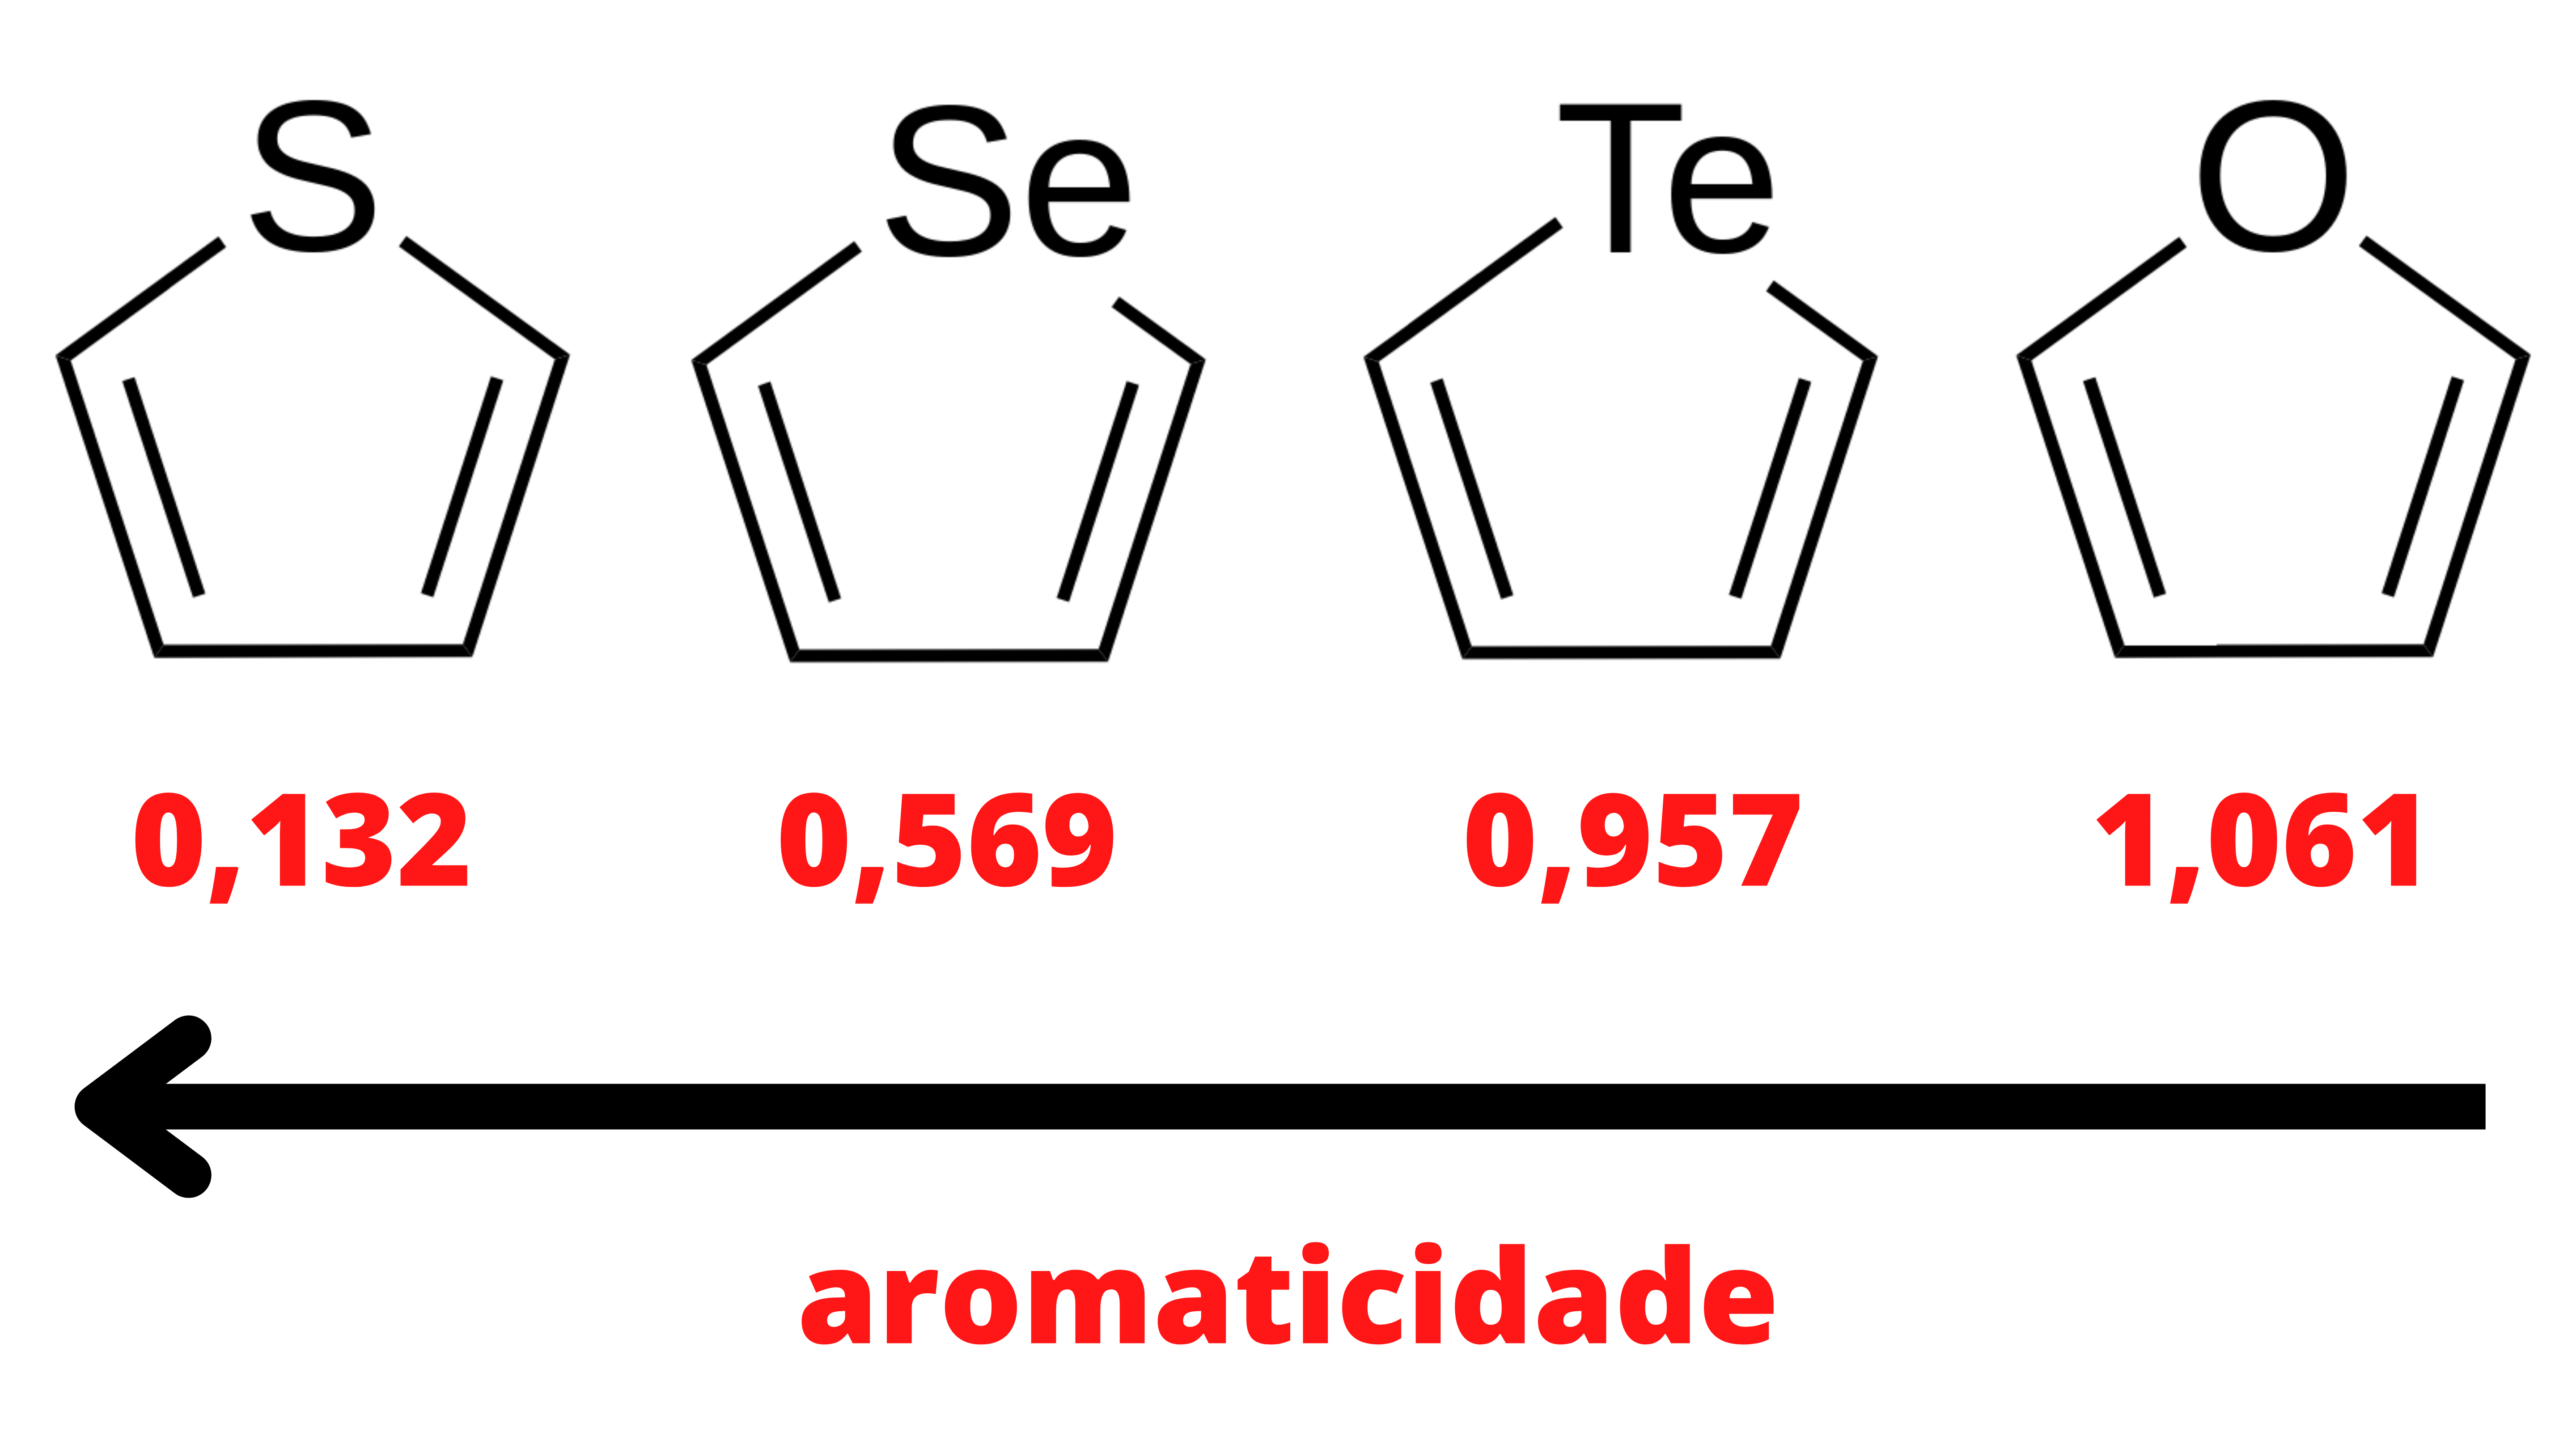
\includegraphics[width=0.45\textwidth]{images/aromaticity(1).png}
	\end{center}
	\fonte{Autor(a). Os valores foram comparados com aqueles obtidos por Fringuelli et al.\autocite{Fringuelli1974}.}
\end{figure}

\subsection{Índice de Bird (1985)}

Bird \autocite{Bird1985, Bird1986, Bird1992} utilizou a mesma ideia, substituindo os comprimentos de ligação por ordens de ligação \autocite{Gordy1947}, mostrado na \autoref{eq:5}. Foi definido então que o coeficiente de variação para as ordens de ligação de um sistema heterocíclico é dado pela \autoref{eq:bird}.

\begin{equation}
\label{eq:bird}
    V = \frac{100}{N_{av}} \sqrt{\displaystyle \frac{\displaystyle \sum (N - N_{av})^2}{n}}
\end{equation}

No caso de um sistema heterocíclico totalmente deslocalizado, $V$ assumirá o valor 0, enquanto que para sistemas heterocíclicos com ligações simples e duplas alternadas, o valor dependerá do tipo de anel, sendo definido como um sistema não-deslocalizado de Kekulé e denotado por $V_k$. Por exemplo, para os anéis de cinco membros, temos $V_k = 35$; para os anéis de seis membros, $V_k = 33.3$; e para anéis fundidos, $V_k = 35$. A escala desses valores foi redefinida por Bird, calculando os seguintes índices: $I_5$, $I_6$ e $I_{5,6}$, dependendo do tipo de anel heterocíclico considerado.

\begin{equation}
    I = 100 \bigg{(} 1 - \frac{V}{V_k} \bigg{)}
\end{equation}

Em 1992, esse termo transformou-se em um índice unificado, denotado por $I_A$, com base nos valores de energia de deslocalização de Hueckel, os quais são: $2 \beta$ para o benzeno, $2.47 \beta$ para o ânion ciclopentadienil e $3.68 \beta$ para o naftaleno. Desse modo, o índice unificado foi definido como: $I_A = I_6 = 1.235 I_5 = 1.34 I_{6,6} = 2.085 I_{5,6}$. Apesar disso, esse método ainda descreve muito mal os sistemas que contenham comprimentos de ligação equalizados, como o próprio benzeno, que continua sendo tão aromático quanto um radialeno de acordo com esse descritor.

\subsection{O modelo do oscilador harmônico}

O próximo passo foi feito modificando a ideia de Julg, substituindo o comprimento de ligação médio ($R_{av}$) da \autoref{eq:1} por um valor conceitual, denominado o comprimento de ligação ótimo ($R_{opt}$)\footnote{No artigo original\autocite{Kruszewski1972}, esse valor é denotado por $d$}. Tal modelo baseia-se no fato de que a energia do oscilador harmônico relativa à extensão ou compressão de uma ligação química depende das constantes de força, diretamente relacionada aos comprimentos dessa ligação. Ou seja, $R_{opt}$ (\autoref{eq:2}) representa a medida da ligação cujo valor de energia requerido para estirá-la até o comprimento de uma ligação simples ou constringir até o comprimento de uma ligação dupla. Desse modo, os comprimentos das ligações CC no etano e no eteno foram tomadas como valores de referência, assumindo que a relação entre as constantes de força para ligações simples e duplas é 2:1.

\begin{figure}[htb]
    \vspace{3\baselineskip}
\begin{equation}
    \label{eq:2}
    R_{opt} = \frac{ \tikzmarknode{single}{ \highlight{blue}{$R_{C-C}$}} + 2 \tikzmarknode{double}{ \highlight{red}{$R_{C=C}$}}}{3} = 1.40 \textit{\AA}
\end{equation}
\begin{tikzpicture}[overlay,remember picture,>=stealth,nodes={align=left,inner ysep=1pt},<-]
    \path (single.north) ++ (-1,1.5em) node[anchor=south east,color=blue!67] (scalep){\textit{$R_{C-C} = 1.53$} \AA};
    \draw [color=blue!87](single.north) |- ([xshift=-3em,color=blue]scalep.south west);
    
    \path (double.north) ++ (1,1.5em) node[anchor=south west, color=red!67] (scalep){\textit{$R_{C=C} = 1.34$} \AA};
    \draw [color=red!87](double.north) |- ([xshift=3em,color=red]scalep.south east);
    
    \path (single.south) ++ (-1,-1.5em) node[anchor=north east,color=blue!67] (scalep){\textit{etano}};
    \draw [color=blue!87](single.south) |- ([xshift=-3em,color=blue]scalep.north west);
    
    \path (double.south) ++ (1,-1.5em) node[anchor=north west, color=red!67] (scalep){\textit{eteno}};
    \draw [color=red!87](double.south) |- ([xshift=3em,color=red]scalep.north east);
\end{tikzpicture}
\end{figure}

O valor obtido pela \autoref{eq:2} apresenta uma boa concordância com o valor experimental obtido para o benzeno (1.398 \AA) \footnote{Esse valor foi medido através de difração de raio X a 10 K\autocite{Stewart1991}.}. A fórmula para o \gls{HOMA} está abaixo:

\begin{figure}[htb]
    \vspace{2\baselineskip}
\begin{equation}
    \label{eq:3}
    \tikzmarknode{HOMA}{\highlight{red}{HOMA}} = 1 - \frac{\tikzmarknode{norm}{\highlight{blue}{$\alpha$}}}{n} \sum_i^n (R_{opt} - R_i)^2
\end{equation}
\begin{tikzpicture}[overlay,remember picture,>=stealth,nodes={align=left,inner ysep=1pt},<-]
    \path (norm.north) ++ (1,1.5em) node[anchor=south west,color=blue!67] (scalep){\textit{$\alpha = 98.89$}};
    \draw [color=blue!87](norm.north) |- ([xshift=3em,color=blue]scalep.south east);
    
    \path (HOMA.north) ++ (-0.70,1.5em) node[anchor=south east,color=red!67] (scalep){\textit{(aromático perfeito) = 1}};
    \draw [color=red!87](HOMA.north) |- ([xshift=-0.70em,color=red]scalep.south west);
    
    \path (HOMA.south) ++ (-1,-1.5em) node[anchor=north east,color=red!67] (scalep){\textit{(não aromático) = 0}};
    \draw [color=red!87](HOMA.south) |- ([xshift=-1.65em,color=blue]scalep.north west);
\end{tikzpicture}
\vspace{1\baselineskip}
\end{figure}

A \autoref{eq:3} pode ser analiticamente convertida na \autoref{eq:4} \autocite{MarekKrygowski1998}. 

\begin{figure}[htb]
    \vspace{2\baselineskip}
\begin{equation}
    \label{eq:4}
    HOMA = 1 - \tikzmarknode{en}{\highlight{blue}{EN}} - \tikzmarknode{geo}{\highlight{red}{GEO}}
\end{equation}
\begin{tikzpicture}[overlay,remember picture,>=stealth,nodes={align=left,inner ysep=1pt},<-]
    \path (en.north) ++ (1,1.5em) node[anchor=south west,color=blue!67] (scalep){\textit{$\alpha(R_{opt} - R_{av})^2$}};
    \draw [color=blue!87](en.north) |- ([xshift=3em,color=blue]scalep.south east);
    
    \path (geo.south) ++ (-1,-1.5em) node[anchor=north east,color=red!67] (scalep){\textit{$\displaystyle \frac{1}{n} \sum_i \alpha(R_{av} - R_i)^2$}};
    \draw [color=red!87](geo.south) |- ([xshift=-1.65em,color=red]scalep.north west);
\end{tikzpicture}
\vspace{2\baselineskip}
\end{figure}

Os componentes EN e GEO representam uma diminuição da aromaticidade devido ao aumento da alternação do comprimento de ligação, fornecendo informações mais detalhadas a respeito da aromaticidade. Enquanto o valor de EN revela quanto o comprimento médio desvia do ótimo, o GEO indica quanto o individual desvia da média. Note que, no caso do benzeno, por exemplo, todos os comprimentos de ligação são iguais, anulando ambos os termos e nos dando um valor de \gls{HOMA} igual a 1, que é considerado \textit{perfeitamente aromático}. Essa normalização é feita pelo fator $\alpha$ presente na \autoref{eq:4}, que funciona somente para compostos carbocíclicos.

No entanto, uma modificação foi realizada em 1993 para abranger no índice HOMA para torná-lo aplicável a sistemas que contenham heteroátomos, representando-as por números de ligação de Pauling. Inicialmente, o mesmo valor de $\alpha$ para as ligações \ce{CC} ($98.89$) foi aplicado para as ligações \ce{CX}, onde \ce{X} são heteroátomos. O $R_{opt}$ foi calculado de acordo com a \autoref{eq:rHOMA}, onde $R_s$ e $R_d$ são os comprimentos de ligação de referência para as ligações simples e duplas, respectivamente, e $\omega$ é a razão das constantes de força para ligações duplas e simples.

Como referência, o comprimento da ligação \ce{C-C} no etano, \ce{C-N} na metilamina, e \ce{C-O} no metanol foram tomados como valores de $R_s$. De forma complementar, a ligação \ce{C=C} no eteno, \ce{C=N} na metilimina, e \ce{C=O} no formaldeído passaram a ser adotadas como as medidas padrão de $R_d$. Desse modo, foi criado o índice \gls{rHOMA} (veja a \autoref{eq:rHOMA}), levando em conta das coordenadas de ressonância.


\begin{figure}[htb]
    \vspace{2\baselineskip}
\begin{equation}
    \label{eq:rHOMA}
    rHOMA = 1 - \frac{\tikzmarknode{alphah}{\highlight{blue}{$\alpha$}}}{n} \sum (\tikzmarknode{ropt}{\highlight{red}{$R_{opt}$}} - R_i)^2
\end{equation}
\begin{tikzpicture}[overlay,remember picture,>=stealth,nodes={align=left,inner ysep=1pt},<-]
    \path (alphah.north) ++ (1,1.5em) node[anchor=south west,color=blue!67] (scalep){\textit{$\alpha = \displaystyle \frac{2}{(R_o - R_s)^2 + (R_{opt} - R_d)^2}$}};
    \draw [color=blue!87](alphah.north) |- ([xshift=3em,color=blue]scalep.south east);

    \path (ropt.south) ++ (1,-1.5em) node[anchor=north west,color=red!67] (scalep){\textit{$R_{opt} = \displaystyle \frac{R_s + \omega R_d}{1 + \omega}$}};
    \draw [color=red!87](ropt.south) |- ([xshift=3em,color=red]scalep.north east);
\end{tikzpicture}
\vspace{2\baselineskip}
\end{figure}

De acordo com a \autoref{eq:rHOMA}, os valores da constante de normalização $\alpha$ para cada tipo de ligação varia de 57.21 (\ce{NO}), 93.52 (\ce{CN}), 94.09 (\ce{CS}), 118.91 (\ce{CP}), 130.33 (\ce{NN}), 157.38 (\ce{CO}), até 257.7 (\ce{CC}) \autocite{Krygowski2000, krygowski2001}. Apesar dos ajustes feitos no índice original do \gls{HOMA}, o \gls{rHOMA} forneceu valores incoerentes para alguns sistemas heterocíclicos aromáticos. Por exemplo, \gls{rHOMA} é próximo de 0 para o furano ($-0.181$) e perto de 0.5 para o pirrol, embora o conhecimento em físico-químico permita inferir que esses valores deveriam ser próximos a 1.

Em 2010, Raczyńska et al.\autocite{Raczyska2010} introduziu o índice \gls{HOMED}. Suas modificações em relação ao \gls{rHOMA} foram feitas ao utilizar os métodos de química quântica para estimar os comprimentos de ligação para moléculas de referência, modificando, consequentemente, os valores de $\alpha$. Os autores argumentam que, utilizar o mesmo nível de teoria para otimizar as geometrias dos sistemas de referência e dos sistemas heterocíclicos tem a vantagem do cancelamento de erros durante a estimativa do \gls{HOMED}.

\section{Aplicações dos critérios geométricos}

No início, a aromaticidade estava fortemente relacionada à reatividade, uma vez que os compostos aromáticos não são somente considerados menos reativos, mas compostos que preferivelmente reagem via mecanismo de substituição, ao invés da adição. Nas espécies policíclicas, as observações podem ser experimentalmente documentadas pela estimativa da basicidade relativa a posições particulares em hidrocarbonetos benzenoides.

Uma discussão qualitativa do caráter aromático de um anel particular em uma molécula de um hidrocarboneto policíclico benzenoide é oferecida pelas regras de Clar. Essas regras classificam os aneis de acordo com a estrutura dos seus elétrons $\pi$, podendo nomeá-los de acordo com um sexteto aromático, um anel vazio, anel de migração ou aquela espécie com ligações duplas localizadas, que pode ser facilmente identificada através do cálculo de \gls{HOMA}.




% ----------------------------------------------------------
\chapter{Objetivos}
% ----------------------------------------------------------

% ----------------------------------------------------------
\section{Objetivo Geral}
% ----------------------------------------------------------

 Desenvolver um \textit{software} de interação gráfica capaz de representar a molécula tridimensionalmente através da leitura de dados de coordenadas cartesianas atômicas e assim retornar parâmetros de aromaticidade segundo a metodologia definida pelo usuário. Poderá, portanto, ser utilizado como uma ferramenta de pós-processamento para o cálculo de propriedades eletrônicas. Além disso, também pretende-se implementar métodos semiempíricos de baixo custo computacional (Hueckel e Hueckel estendido) para auxiliar na avaliação e representação dos orbitais atômicos e moleculares.

% ----------------------------------------------------------
\section{Objetivos Específicos}
% ----------------------------------------------------------

\begin{itemize}
    %\item Realizar pré-otimizações de geometria utilizando métodos semi-empíricos e \textcolor{red}{realizando leituras de estruturas obtidas por outros métodos através de outros \textit{softwares}; complementar};
    
    \item Utilizar métodos semiempíricos para avaliar orbitais atômicos e moleculares.
    
    \item Automatizar a leitura de arquivos de saída \textit{outputs} de cálculos de estrutura eletrônica molecular visando extrair dados geométricos para determinar critérios de aromaticidade geométricos em sistemas orgânicos, através de uma interface gráfica.

    \item Utilizar a teoria de grafos para implementar a determinação dos índices HOMA, EN, e GEO; 
    
    \item Realizar \textit{benchmark} dos resultados obtidos com estruturas já reportadas na literatura para fins de  validação e comparação do tempo de computação na metodologia aplicada.
\end{itemize}